\documentclass[sigconf]{acmart}

\usepackage{booktabs} % For formal tables
\usepackage{float}
\usepackage{longtable}
\usepackage{subcaption}
\usepackage{multirow}
\usepackage{tikz}
\graphicspath{{2019_iui_augment/images/}, {2019_iui_augment/auto_fig/}}

%\def\acmBooktitle#1{\gdef\@acmBooktitle{#1}}
%\acmBooktitle{Proceedings of \acmConference@name \ifx\acmConference@name\acmConference@shortname\else \ (\acmConference@shortname)\fi}

\copyrightyear{2019}
\acmYear{2019}
\setcopyright{acmlicensed}
\acmConference[IUI '19]{24th International Conference on Intelligent User Interfaces}{March 17--20, 2019}{Marina del Rey, CA, USA}
%\acmBooktitle{24th International Conference on Intelligent User Interfaces (IUI '19), March 17--20, 2019, Marina del Rey, CA, USA}
\acmPrice{15.00}
\acmDOI{10.1145/3301275.3302265}
\acmISBN{978-1-4503-6272-6/19/03}

\begin{document}
\title{What can AI do for me?}
\subtitle{Evaluating Machine Learning Interpretations in Cooperative Play}

\author{Shi Feng}
\affiliation{%
  \institution{University of Maryland}
  \city{College Park}
  \state{Maryland}
}
\email{shifeng@cs.umd.edu}

\author{Jordan Boyd-Graber}
\affiliation{%
  \institution{University of Maryland}
  \city{College Park}
  \state{Maryland}
}
\email{jbg@umiacs.umd.edu}

\newcommand\BibTeX{B{\sc ib}\TeX}
\newcommand{\qb}[0]{Quizbowl}
\newcommand{\abr}[1]{\textsc{#1}}
\newcommand{\vis}[1]{\emph{#1}}
\newcommand{\etal}[0]{\emph{et al.}}
\definecolor{lightblue}{HTML}{3cc7ea}
\definecolor{periwinkle}{rgb}{0.8, 0.8, 1.0}
\definecolor{colorsquad}{rgb}{0,1,0}
\definecolor{colorsnli}{rgb}{1,0,0}
\definecolor{colorvqa}{rgb}{1,1,0}
\newcommand{\ai}[0]{\textsc{ai}}

\newif\ifcomment\commentfalse
\ifcomment
 \newcommand{\jbgcomment}[1]{ \colorbox{red}{   \parbox{.8\linewidth}{ JBG: #1}  }}
 \newcommand{\fscomment}[1]{ \colorbox{green}{   \parbox{.8\linewidth}{ fs: #1}  }}
\else
\newcommand{\jbgcomment}[1]{}
\newcommand{\fscomment}[1]{}
\fi


\begin{abstract}
Machine learning is an important tool for decision making, but its
ethical and responsible application requires rigorous vetting of its
interpretability and utility: an understudied problem, particularly
for natural language processing models.  
We propose an evaluation of interpretation on a
real task with real human users, where the effectiveness of
interpretation is measured by how much it improves human performance.
We design a grounded, realistic human-computer cooperative setting
using a question answering task, \qb{}.
We recruit both trivia experts and novices to play this game with
computer as their teammate, who communicates its prediction via three
different interpretations.
We also provide design guidance for natural language processing
human-in-the-loop settings.

\end{abstract}

%
% The code below should be generated by the tool at
% http://dl.acm.org/ccs.cfm
% Please copy and paste the code instead of the example below.
%
\begin{CCSXML}
<ccs2012>
<concept>
<concept_id>10003120.10003121.10003124.10010870</concept_id>
<concept_desc>Human-centered computing~Natural language interfaces</concept_desc>
<concept_significance>500</concept_significance>
</concept>
<concept>
<concept_id>10003120.10003121.10003124.10011751</concept_id>
<concept_desc>Human-centered computing~Collaborative interaction</concept_desc>
<concept_significance>500</concept_significance>
</concept>
</ccs2012>
\end{CCSXML}

\ccsdesc[500]{Human-centered computing~Natural language interfaces}
\ccsdesc[500]{Human-centered computing~Collaborative interaction}

\keywords{interpretability; natural language processing; question answering}

\maketitle

\section{Introduction}
\label{sec:intro}

% 1. ML is good, but still need humans
The field of machine learning (\abr{ml}) is making rapid progress,
with models surpassing human performance on many tasks, such as
image classification~\cite{he2015delving}, playing video
games~\cite{mnih2015human}, and playing Go~\cite{silver2017mastering}.
However, a drop-in replacement for humans---even assuming that it is
achievable---is not always the ideal integration of machine learning
into real-world decision making.
In sensitive areas such as medicine and criminal justice, the
computational objectives of \abr{ml} models cannot yet fully
capture the factors one must consider when making a
decision, such as fairness and transparency. In some other areas such
as natural language processing, the
strengths of humans and computers are sometimes complimentary.
Humans are excellent at reasoning about what we
consider ``common sense'', while some tasks in this category such as
disambiguating word senses are still difficult for
computers~\cite{papandrea2017supwsd}.
Tasks like deceptive review detection is difficult and time consuming
for humans while simple linear \abr{ml} models achieve high accuracy
with little processing time~\cite{lai2018human}.
On tasks such as simultaneous interpretation where humans are
still far superior than computers, experts can still be assisted on
some aspects of the task: interpreters often
find certain content such as technical terms, names of people and
organizations, and numbers difficult to translate, while 
computers find that easy.  The integration of \abr{ml}
can be more effective and efficient when humans and computers
cooperate.

% 2. the need for interpretation in cooperation
Cooperation is only effective when the two parties communicate
well with each other. One direction of this communication, from
humans to computers, is well-studied:
\abr{ml} models can be improved with human feedback using
reinforcement learning~\cite{sutton1998introduction} and imitation
learning~\cite{ross2011reduction,ross2018regularizing}. The
other direction of the communication, from \abr{ml} models to
humans, presents different challenges:
a standard classification model outputs a prediction (e.g., an object
class given an image), but without any justification.
% It is often not insightful to look directly at the model's
% internals, which in the case of modern neural networks consist of
% millions of parameters.
Although the prediction can be presented with a confidence score (a
value between zero and one), humans struggle to interpret and act on
numbers~\cite{peters2006numeracy, reyna2008numeracy}; moreover, due to
over-fitting, confidence scores from a neural models can be much
higher than the actual prediction
uncertainty~\cite{guo2017calibration}.

% 3. the role of interpretation
To bridge the gap between human and \abr{ml} models in a cooperative
setting, interpretation methods 
explain the model predictions in a more expressive,
human-intelligible way. In a human-centered setting where humans make
the final decision, these methods help users decide to trust the
model prediction or not. In Section~\ref{sec:related} we discuss the
existing work of interpreting \abr{ml} models.

% 4. evaluation of interpretation is difficult
Progress in \abr{ml} research largely relies on rigorous evaluations,
which often relies on standard
datasets, for example ImageNet~\cite{deng2009imagenet} for image
classification and Penn Treebank~\cite{marcus1993building} for
language modeling.
Although interpretability is valued as a laudable goal, it remains
elusive to evaluate.
We do not have such standard dataset for interpretability---it is not
clear what the ground truth should be. As
Lipton~\cite{lipton2016mythos} argues, there is no clear agreement on what
interpretability means; there is no definitive answer to what
interpretation is most faithful to the model and useful for humans at
the same time. Secondly, it is not realistic to evaluate
interpretability without humans, the eventual consumer of
interpretations~\cite{narayanan2018humans}.
Previous work focuses on how humans can use interpretations to help
the model do its job better; for example, interpretations generated by
Local Interpretable Model-Agnostic
Explanations~\cite[\abr{lime}]{ribeiro2016lime} help humans do feature
engineering to improve downstream predictions of a classifier; in
other work interpretations are used to help humans debug \abr{ml}
models~\cite{ribeiro2018semantically,fong2017interpretable}.

% 5. we take the human-centered perspective
Kleinberg~\etal{}~\cite{kleinberg2017human} propose a different
perspective and ask how \abr{ml} can improve human decision making.
Applying this thinking, we measure
interpretability by asking what \abr{ml} can do
for humans through interpretations: they should
\emph{augment}~\cite{Koedinger-13} human intelligence. This concept
resonates with the seminal work of mixed-initiative user
interface~\cite{horvitz1999principles}, which emphasizes 
user interfaces where the human and the computer can drive towards a
shared goal and ones that enhance human ability~\cite{allen1999mixed}.

% 6. why we focus on forms instead of specific methods
Interpretations come in many forms; we focus on three
popular options among the interpretable \abr{ml} community:
visualizing uncertainty, highlighting
important input features, and retrieving relevant training
examples.  We measure how they help humans on the tasks at hand and
focus on answering the question ``how effective can interpretations
communicate model predictions to humans''. The other question is ``how
faithful an interpretation is to the model''.
Section~\ref{sec:eval_qb} discusses our choice of model to answer the
first question; we leave the second question to future work, but
discuss in Section~\ref{sec:discussion} how our framework, interface,
and experiments can be directly applied.

% 7. introduce QB, forward point qb section
We choose the testbed for our interpretability evaluation from the
natural language domain---a question answering task called
\qb{}~\cite{boydgraber2012besting}.  As we discuss in
Section~\ref{sec:eval_qb}, in addition to being a
challenging task for \abr{ml}, it is also an exciting game that is
loved by human trivia enthusiasts. Furthermore, it is a task where
humans and \abr{ml} have complementary strengths, so effective
collaboration with interpretations has great potential.

% 8. a teaser of what we do
We recruit both \qb{} enthusiasts and turkers from Amazon Mechanical
Turk (novices in comparison) to play \qb{} on an interactive
interface,
provide them different combinations of the interpretations, and
measure how their performance changes.  These different user groups
reveal imperfections in how we communicate the way a computer answers
questions.  Experts have enough world and task expertise to
confidently overrule when the computer is wrong; however, as we will
discuss in Section~\ref{sec:results}, novices are too trusting: they
play more aggressively with computer assistance, but are not able to
discern useful help from the misleading ones as well as the experts.
In Section~\ref{sec:discussion}, we propose how to can explore new
interpretations and visualizations to help humans more confidently
interpret \abr{ml} algorithms.

\section{Related Work}
\label{sec:related}

\subsection{Human-AI Cooperation}
% 1. usability of ai is a concern
Explainability is a central problem of applied \abr{ai}, with research
stretching back to the days of expert
systems~\cite{swartout1983xplain}.
% Early work exposes the potential lack of usability of \abr{ai}:
% Suchman~\cite{suchman1987plans} criticizes that \abr{ai}'s rigid
% concepts of ``plans and goals'' are incompatible with how people
% behave in the real world.
The recent surge of interest in this area is the
result of the success of \abr{ml} models based on neural networks,
a.k.a.\ deep learning~\cite{lecun2015deep}. These complicated models
have stupendous predictive power, but at the same time brittle, best
demonstrated by the existence of adversarial
examples~\cite{goodfellow2014explaining}, where small perturbation to
the input leads to significant change in the model output.
From a practical standpoint, the inscrutability of these models makes
it difficult to integrate into real world decision-making in high risk
areas such as urban planning, disease diagnosis, predicting insurance
risk, and criminal justice.
The fairness, accountability, and transparency of machine learning
remain a concern~\cite{acm2017public}, which is reflected in the
``right to explanation'' in European Union's new General Data
Protection Regulation~\cite[\abr{gdpr}]{gdpr}. 

% 2. importance of interpretation
Thus, \abr{ml} model predictions need explanations.
Efforts including the Explainable \abr{ai} (\abr{xai})
initiative~\cite{gunning2017explainable} led to the conceptualization
of a series of human-\abr{ai} cooperation paradigms, including
human-aware \abr{ai}~\cite{chakraborti2017ai}, and human-robot
teaming~\cite{vinson2018human}. 
As an example, Schmidt and Herrmann~\cite{schmidt2017intervention}
recognize the importance of interpretability when interacting with
autonomous vehicles.
Such need motivated the \abr{ml} community to develop interpretation
methods for deep neural models~\cite[\em inter
alia]{baehrens2010explain, simonyan2013deep}.

% 3. moved to next subsection

% 4. previous hci work on evaluation of interpretation
The \abr{hci} community has a rich body of research towards making
computers more usable, for example in interaction
design~\cite{ju2008design} and software
learnability~\cite{grossman2009survey}.
To borrow insights from the human side,
Miller~\cite{miller2017explanation} provides an overview of social
science research regarding how people define, generate, select,
evaluate, and present explanations.
Still, interpreting \abr{ml} models has its unique challenges.
Krause~\etal{}~\cite{krause2016interacting} compare different \abr{ml}
models under one visualization method, partial dependency.
Smith~\etal{}~\cite{smith2017evaluating} and
Lee~\etal{}~\cite{lee2017human} focus on the
interpretation of topic models. In contrast, we compare interpretation
of classification models across various forms, making
our framework more generalizable to other tasks and interpretation
methods.

\subsection{Interpretation of Machine Learning Models}

% 5. forms interpretations
Interpretations can take on several different forms.
We focus on interpretation in the form of uncertainty, important
input features, and relevant training examples.  Some \abr{ml} models
provide canonical interpretations.
% For the sparse linear classifier
% used in \abr{lime}~\cite{ribeiro2016lime}, important input features
% can be identified by inspecting the coefficients.
For models such as
decision trees and association rule
lists~\cite{lakkaraju2016interpretable, letham2015interpretable}, the
interpretation is built in the prediction itself.  However, most
state-of-the-art models in vision and language---domains with the
widest range of applications---are deep neural models with hundreds of
thousands of parameters. Next we introduce previous work on
interpreting both simpler linear models and more complicated neural
networks, in each of the three forms.

% 6. uncertainty
\paragraph{Conveying Uncertainty}
Augmenting the prediction from a neural network classifier with a
confidence score (a value between zero and one) conveys the
uncertainty of the model. In a cooperative setting, the uncertainty
helps humans decide to trust the model or
not~\cite{antifakos2005towards, rukzio2006visualization}. To make it
more informative, we can also display the confidence for the
classes other than the top one~\cite{liu2017towards}.
Confidence of simple linear models are usually
well-calibrated, but estimating uncertainty for a deep neural model
is challenging: due to overfitting, they are over-confident 
and require careful calibration~\cite{guo2017calibration,
feng2018rawr}.
% Sometimes uncertainty estimate needs to be combined with anomaly
% detection to be robust~\cite{hendrycks2016baseline,feng2018rawr}.

% 7. input features
\paragraph{Highlighting Important Features}
Model predictions can be explained by
highlighting the most salient features in the input, typically visualized
by a heat map.  For a linear classifier, the most salient features
are the ones with the largest corresponding coefficients;  For
non-linear classifiers, the relevance of a feature can be calculated
by the gradient of the loss function w.r.t.\ that
feature~\cite{simonyan2013deep}.
Alternatively, one can locally approximate a non-linear classifier
with a simpler linear model, then use the coefficients to explain the
predictions from the non-linear model~\cite{ribeiro2016lime}.

% 8. training examples
\paragraph{Interpretation by Example}
We can explain a prediction on a test example by finding the most
influential training examples.  Various metrics exist for finding
important training examples, such as distance in the representation
space which is natural to linear models, clustering algorithms and
their deep variation~\cite{papernot2018dknn}, and influence
functions~\cite{koh2017influence} for non-linear models.

As we discuss in Section~\ref{sec:eval_qb}, although our experiments
use a linear classifier,  our method can be generalized to evaluating
these methods designed for neural models
(Section~\ref{sec:discussion}).

\subsection{Evaluation of Interpretation}

% 3. interpretation evaluation is difficult
A fair and accurate assessment of interpretations is crucial for
improving the understability of \abr{ai} and consequently
human-\abr{ai} cooperation.
Although interpretation methods have rigorous mathematical
formulations, some even axiomatically
derived~\cite{sundararajan2017axiomatic}, it remains unclear how we
can evaluate the efficacy of these methods on \emph{real tasks} with
\emph{real users}. Lipton~\cite{lipton2016mythos} argues that there is no
clear agreement on what interpretability means: looking at \abr{ml}
models alone, no definitive answer exists as in what would be the best
interpretation in both faithfulness to the model and usefulness
to humans.

% 9. interpretation evaluation is important
As it is widely accepted that machine learning models should be
evaluated beyond natural examples, e.g., in adversarial
settings~\cite{goodfellow2014explaining, jia2017adversarial},
the evaluation of interpretation should not be limited to being
visually pleasing. Indeed, interpretations can be fragile under small
input perturbations~\cite{ghorbani2017interpretation,
kindermans2017unreliability}, unfaithful to the
model~\cite{hooker2018evaluating, adebayo2018sanity, feng2018rawr},
and create a false sense of security~\cite{jiang2018trust}.

% 10. finale's work on interpretation evaluation
Conditioning a more realistic setting, Doshi-Velez and
Kim~\cite{doshivelez2017towards}
provide an ontology of various evaluations of interpretation with a
human in the loop. Following this framework,
Narayanan~\etal{}~\cite{narayanan2018humans} conduct
one such evaluation with synthetic tasks and hand-crafted
interpretations to study their desirable cognitive properties.

% 11. overview of what we do
We focus on \emph{application-grounded} evaluation---real tasks with
real users.  This setting best aligns with what interpretations are
intended for---improving human performance on the end task.  However,
application-grounded evaluation is also challenging because it
requires real tasks and motivated real users. The task needs a large
pool of willing human testers, and ideally one that challenges both
humans and computers. As we discuss in the next section, \qb{} is a
task that satisfies these conditions.

\section{Interpretation Testbed: Quizbowl}
\label{sec:eval_qb}

% 1. lead-in
This section introduces \qb{}, our testbed for evaluating the three
forms of interpretations. We discuss how the task suits our purposes,
which model to use, and how we generate the interpretations.

\subsection{\qb{} and Computer Models}

% 2. overview of the task
\qb{} is both a challenging task for
machine learning~\cite{boydgraber2012besting} and a trivia game played
by thousands of students around the world each year. Each question
consists of multiple clues, presented to the players
\emph{word-by-word}, verbally or in text.
The ordering of \qb{} clues is
\emph{pyramidal}---difficult clues at the beginning, easy clues at the
end, and the challenge is to answer with as few clues as possible.
For a question with $n$ words, the players have $n$ chances to decide
that \emph{this is all the information I need to answer the question}.
The player can do so by \emph{buzzing} before the question is fully
read, which interrupts the readout so
the player provide an answer. Whoever gets the answer correct first
wins that question and receives ten points.\footnote{Like previous
work, we only consider \emph{toss-up}/\emph{starter} questions.} But
when players buzz and answer incorrectly, they lose five points.
Success in \qb{} requires a player to not only be knowledgeable but
also balance between aggressiveness and
accuracy~\cite{he2016opponent}.

% 6. qb challenges computers and humans in different ways
\qb{} challenges humans and computers in different
ways~\cite{boydgraber2012besting, wallace2018trick}.  Computers can
memorize every poem and book ever written, making it trivial to
identify quotes.  Computers can also memorize all of the \emph{reflex
clues} that point to answers (e.g., if you hear ``phosphonium ylide'',
answer \underline{Wittig}) and apply them without any higher reasoning.
Humans can chain together evidence (``predecessor of the Queen who
pardoned Alan Turing'') and solve wordplay (``opera about an enchanted
woodwind instrument'').  
Thus, \qb{} is representative of tasks where human-computer
cooperation 
has huge potential~\cite{Thompson-13}. This also makes \qb{} a
suitable testbed for interpretation methods designed to better
interface humans and computers.

Thus, instead of trying to beat humans with computers, we team
them together and use their cooperation to
measure the effectiveness of interpretations.  In our cooperative
setting, instead of having a model to decide when to buzz in,
\emph{the human needs to decide when the system has a good guess}.
When answering a \qb{} question---which takes many steps, the human
constantly interacts with the model, which provides many opportunities
to evaluate the interpretability of models.  Every word provides new
evidence that can change the underlying interpretation and convince
the human that the system has a good answer to offer.
Furthermore, the competitiveness of
\qb{} encourages humans to use the help from the computers as much as
possible, avoiding a degenerate scenario where the users solve the
task on their own. It also attracts a large pool of enthusiastic
participants, which is crucial for application-grounded evaluations.
Sesction~\ref{sec:setup} discusses the cooperation in detail.

% \jbgcomment{Not too important for IUI, but I would reframe as a linear
% decision function and you can talk about the feature set.  This would
% be useful for when we share it with ML researchers.}

% 3. model
As mentioned in Section~\ref{sec:intro}, we focus on the comparison
between three forms of interpretation, using one method for each form.
But which method to use?  Linear models provide canonical
interpretations: important features and relevant training examples can
be identified based on the coefficients. On the other hand, neural
models do not have
canonical interpretations: 
all interpretations are approximations, which by definition are not
completely faithful to the model~\cite{rudin2018please}.
% To avoid conflating the faithfulness with usefulness, we choose a
% linear model for our experiments.

Luckily in the case of \qb{}, we have linear models with
performance on par or better than neural models.
\abr{qanta}~\cite{iyyer2014ann} is a simple, powerful, and
interpretable system for \qb{}. A stripped-down, minimal version of it
is provided to participants in the \abr{nips} 2017 Human-Computer
Question Answering competition~\cite{nips2018qbcomp}.  We use the
\emph{guesser} of \abr{qanta}, which has a linear decision function
built on ElasticSearch~\cite[\abr{es}]{gormley2015es}.  As the name
implies, guesser generates guesses for what the answer to a question
could be.  Despite its simplicity, \abr{es}-based
systems perform very well on \qb{}, defeating top trivia
players.\footnote{\url{https://youtu.be/bYFqMINXayc}}

\subsection{Interpretation of a Question Answering Model}

% talk again about the choice of linear model here

% 9. maybe merge with the previous one
Our goal is to see which forms of interpretation are most
helpful to the users, and a linear model with natural
interpretations makes this easy.  Our \abr{es}-based \qb{} model
supports three forms of interpretations, each corresponding to a class
of methods widely studied in recent literature as mentioned in the
previous section.
Given a question never seen in the training set, \abr{es} mainly uses
tf-idf features to find the
most relevant training example, which is either a Wikipedia page or a
previously seen \qb{} question, and then uses the label of that
document as the answer.

% 10. how to get scores
To convey the uncertainty of model predictions, we augment the top ten
guesses from our model with their corresponding scores. 
Unlike regular classification models, \abr{es} does not output 
a probability distribution over all possible answers.  Its scores
measure the relevance between the question and training examples, but
are not normalized.
We keep the scores unnormalized to stay true to the model.
Despite its simplistic form, these scores provide strong
signal about model uncertainty, for example, a large gap between the
top two scores usually indicate a confident prediction.
% The buzzer module of \abr{qanta}, whose job is decide when to buzz in,
% relied on only these scores to defeat top human
% players~\cite{nips2018qbcomp}.

% 11. how to get important input features
Interpretation by example---getting the \emph{evidence}---is
straightforward with our \abr{es}-based model.
The prediction is the label of the most relevant documents, so
the extracted documents are naturally the most salient training
examples.  We can further identify the most important words in each
retrieved training example, using the highlight
\abr{api}\footnote{\url{https://www.elastic.co/guide/en/elasticsearch/reference/current/search-request-highlighting.html}}.
This gives us \emph{evidence highlights}.
The player can make a better decision of whether to trust the computer
prediction by judging how relevant the evidence is to the question.

% 12. how to get training examples
To highlight important input features---generating \emph{question
highlights}---we build on the previous \emph{evidence highlights}.
The most
important words in the question naturally emerge when we compare the
question against the most salient training example.  Specifically, we
go through the question and find words that appear highlighted in the
evidence. Question highlights inform the player whether the computer
is looking at the right keywords in the question.

Although generating \emph{question highlights} depends on
\emph{evidence highlights}, the former can be displayed without the
later. We discuss how we control which interpretation to display in
the next two sections.

\begin{figure*}[t]
\centering
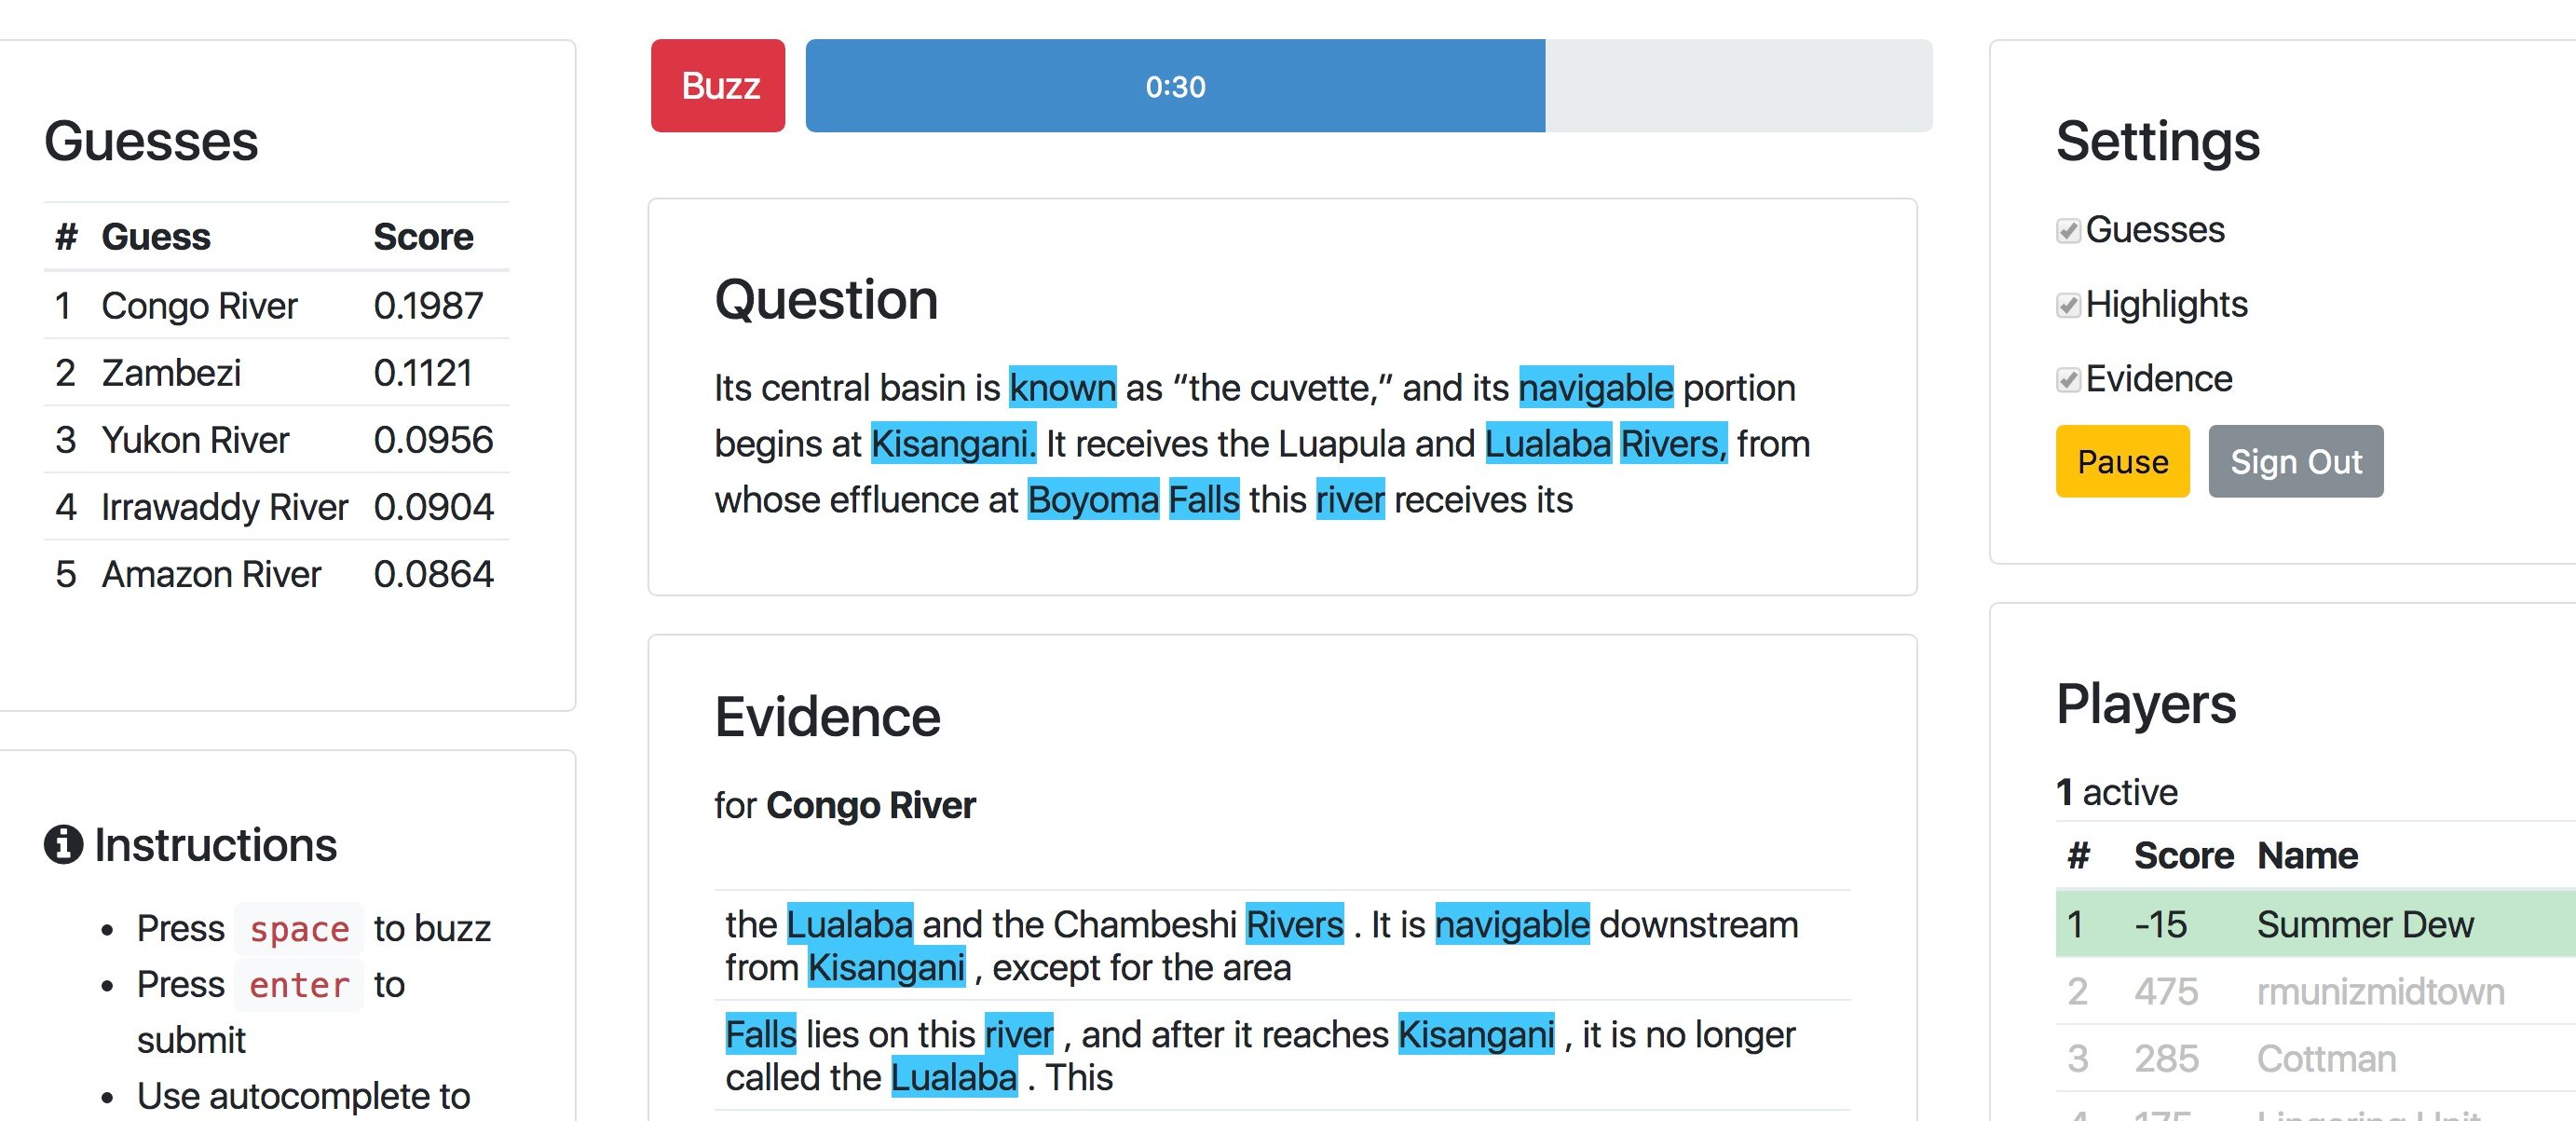
\includegraphics[width=0.85\textwidth]{screenshot_all}
\caption{\label{fig:screenshot} Screenshot of the interface. Question is
    displayed in the middle area word-by-word, with question highlights
    displayed in the same panel. Guesses are listed in the panel on the left.
    Evidence is in the panel below.}
\end{figure*}

\section{Interface Design}
\label{sec:design}

% 1. lead-in
We design our \qb{} interface (Figure~\ref{fig:screenshot}) to
\emph{visualize} the three interpretations described in the previous
section. This section introduces the visualizations, placement, and
interactivity of the interface. 

% 2. design principle
To make \qb{} players feel at home, we follow the general framework
of~\url{Protobowl.com}, a popular \qb{} platform
% inspired by Boyd-Graber~\etal{}~\cite{boydgraber2012besting} 
that many
players actively use for practice.  The \textbf{Question} area is
in the center, and the question is displayed word-by-word in
the text box. A \textbf{Buzz} button is located close above the
question area, and to further reduce the distraction from the question
area, players can also buzz in using the space key. After buzzing, the
player have eight seconds to enter and select an answer from
a drop-down menu.

\begin{figure}[H]
\centering
\fbox{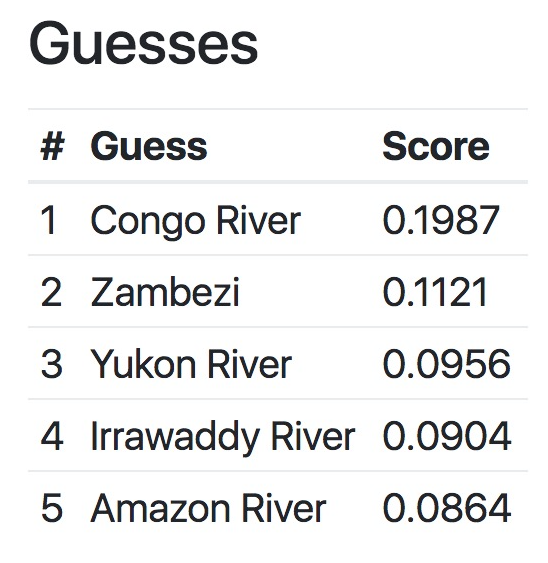
\includegraphics[width=0.4\columnwidth]{screenshot_guesses}}
\end{figure}

% 3. guesses
\textbf{Guesses} show the answers the computer is considering along
with the associated score.  Top ten answers are sorted according to
their score (the system prefers higher scores).  This helps convey
when the model is uncertain (e.g., if all of the guesses have a low
score).

\begin{figure}[H]
\centering
\fbox{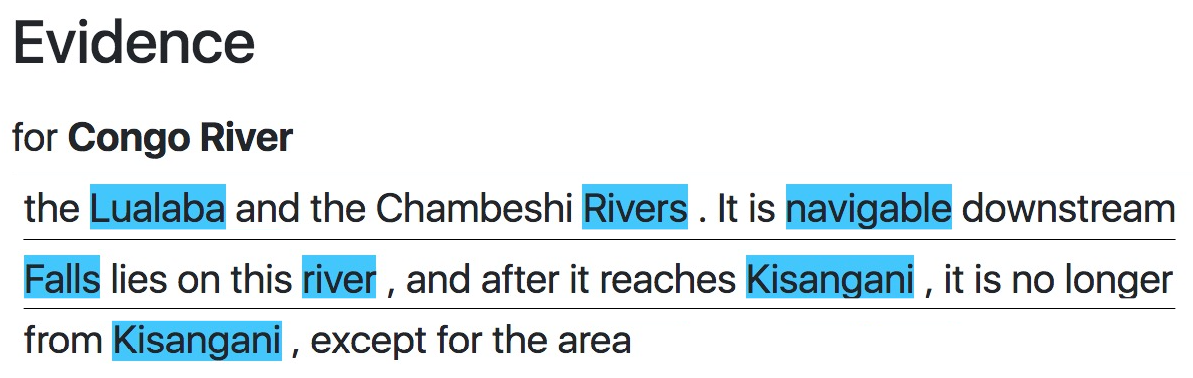
\includegraphics[width=0.85\columnwidth]{screenshot_evidence}}
\end{figure}

% 4. evidence
To inform the player of how the model's prediction is supported by
training examples, \textbf{Evidence} shows the relevant snippets of
the most salient training examples for the top guess. It is located
below the question area and has the same width to provide a direct
comparison against the input question. Each line of the text area
shows the snippet of one selected document.

\begin{figure}[H]
\centering
\fbox{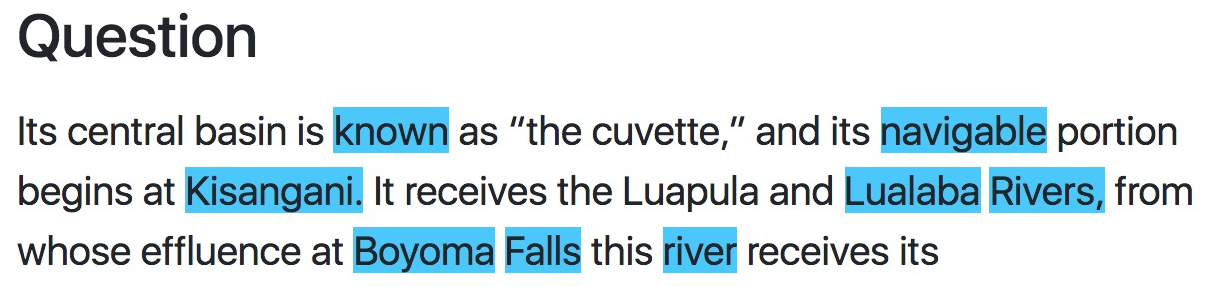
\includegraphics[width=0.85\columnwidth]{screenshot_highlight}}
\end{figure}

% 5. highlight
We use \textbf{Highlight} to visualize the most salient words in both
the input question and the evidence snippets. These words are selected
for the top guess. As introduced in the previous section, we first
highlight important words in the training example snippets using an
\abr{api} of \abr{es}, then find their appearances in the input and
highlight those too. 

% \jbgcomment{This is very unclear.  Rewrite, use concrete words
% (instead of ``visualize''.  Give example, and use ``evidence
% highlight'' and ``question highlight'' if you're going to have two
% terms.}

% 6. combinations, need to expand
Multiple interpretations can be shown in combination. The
combination of highlight and evidence has a compounding effect: when
both are enabled, players see highlighted words in both the question
and the evidence (for example in Figure~\ref{fig:screenshot});
when highlight is enabled without evidence, players only see
highlights in the question.

% \jbgcomment{The below paragraph makes it seem like we're trying to
%   make highlights win.  Say that it needs to be the same width as
%   question, so we place it below.  Then say that we discuss this
%   choice in the limitations section at the end of the paper.}

% 7. hint on UI future work
Our design goal is to minimize distraction from the
question area while boosting the competitiveness of the player. So we place
the question area in the middle and have all interpretations around it.
% This might give highlight visualization an unfair amount of
% attention, since it is in a more central position.
It is difficult to ensure that different forms of
interpretations are exposed to the users equally, as some forms (e.g.,
evidence) are inherently less intuitive to visualize. However,
all interpretations must be implemented in an interface for a
real-world evaluation; we discuss the limitations of our design and
future work in Section~\ref{sec:discussion}.

\section{Setup}
\label{sec:setup}

% 1. overview:
%   reiterate that we eval viz by human performance
%   briefly say how they cooperate
%   briefly say how we control viz
% This section explains how we use our interface to evaluate the
% interpretations introduced in the previous section. 
This section explains how human players and the computer guesser play
in cooperation. To ensure accuracy and unbiasedness, we control what
interpretations each player sees instead of letting them choose.

\subsection{Data and Participants}

% 2. data
We collect 160 new questions for this evaluation that had not been 
previously seen by the \qb{} community to avoid bias in players'
exposure to questions.

% 3. participants
We recruit 40 experts (\qb{} enthusiasts) by advertising on an
online forum, and 40 novices using MTurk. Experts are
free to play as many questions as they want (but each player can only
play a question once), and we encourage them to play more by offering
monetary prizes for those who finish the whole question set. We
require novices to each answer at least twenty questions and require
a positive score at the end (according to standard \qb{} scoring
rules) to encourage good faith responses. Online \qb{} platforms such
as \url{Protobowl.com} are usually anonymous, so we do not collect
any information about the participants other than an email
address for collecting prizes (optional).

\subsection{Human-AI Cooperation on \qb{}}

% 4. how they team up
Unlike previous work where \qb{} interfaces are used for computers to
\emph{compete} with
humans~\cite{boydgraber2012besting,he2016opponent}, our interface aims
at human-\abr{ai} \emph{cooperation}. We let a human player form a
team with a computer teammate and put the human in charge.  As the
question is displayed word-by-word, the computer periodically updates
its guesses and interpretations (every 4 words in our experiments); at
any point before the question is fully read, the human can decide to
buzz, interrupt the readout, and provide an answer. The
interpretations should help the human better decide whether to
trust the computer's prediction or not.

% 5. lead-in to expert vs novice
We have two different experimental settings. In the simpler,
non-competitive \textbf{novice setting}, we have a single turker
interact with the interface, with the computer guesser
as teammate, but without opponents.
% For the novice setting, we recruit workers on Mechanical Turk.

% 6. expert 1
The competitive \textbf{expert setting} better resembles real \qb{}
games, and the players in this setting are experts
that enjoy the game.
To encourage them to play to the best of their ability, we
simulate the \qb{} setting as closely as possible (for novices the
simple task is already taxing enough without competition).  In a real
\qb{} match, players not just compete against themselves (can I get
the question right?) but also with each other (can I get the question
right before Selene does?).  \qb{}'s pyramidality
encourages competition: difficult clues at the start of the
question help determine who knows the most about a subject.
Our interface resembles \url{Protobowl.com}, a popular online \qb{}
platform where players play against each other (but
without the computer teammate).  The computer generates the same
output (both prediction and interpretations), but human players might
have access to different interpretations, e.g., David sees evidence while
Selene sees question highlights. Next section discusses the setup in
detail. 
% The competitiveness of the expert setting is familiar to \qb{}
% enthusiasts, whom we recruit via a \qb{} community forum.

% 8. community effort
Our experiment in the expert setting was possible thanks to \qb{}'s
enthusiast community. It was because \qb{}ers love to play this game
and to improve their skills by practicing, that they were willing to
learn our interface, team up with the computer, and compete under this
slightly irregular setting.  This provided us new perspectives of how
users from a wider range of skill levels use interpretations,
compared to many previous work that only had non-expert
turkers~\cite{smith2017evaluating,kneusel2017improving,clark2018creative}.

\subsection{Controlling Which Interpretations to Show}

% 9. lead-in to controlling interpretations, need rework
Each of the three interpretations can be turned on or off, so we have
in total $2\times2\times2=8$ conditions, including the null condition
where all interpretations are hidden.
To compare within-subjects (players vary greatly based on their innate
ability), we vary the interpretations a player sees randomly.  We
sample the enabled combination with the goal of having, in
expectation, a uniform distribution over players, questions, and
interpretation combinations. For player $P$ at question $Q$, we sample
from an eight-class categorical distribution, with the parameter of
each combination~$C$ set to $N-\#(C, P)$, where $\#(C, P)$ is the
number of times player~$P$ has seen the interpretation combination~$C$
and $N$ is the expected count of each combination (in our case 
the number of questions divided by eight).  In the expert setting,
interpretations are sampled independently for each player, and players
may (and usually do) see different interpretations.
For all experiments, we only allow each player to answer each question
once.

\section{Results}
\label{sec:results}

% \begin{table*}[t]
% \centering
% \begin{tabular}{llll}
% Guesses & \includegraphics[width=0.5\columnwidth]{ecoef_g} \\
% Highlight & \includegraphics[width=0.5\columnwidth]{ecoef_h} & \includegraphics[width=0.5\columnwidth]{ecoef_gh} \\
% Evidence & \includegraphics[width=0.5\columnwidth]{ecoef_e} & \includegraphics[width=0.5\columnwidth]{ecoef_ge} & \includegraphics[width=0.5\columnwidth]{ecoef_he}\\
% All & \includegraphics[width=0.5\columnwidth]{ecoef_all}\\
% \end{tabular}
% \end{table*}

\begin{figure}[t]
    \centering
    \textbf{Effect of interpretations}\par\medskip
    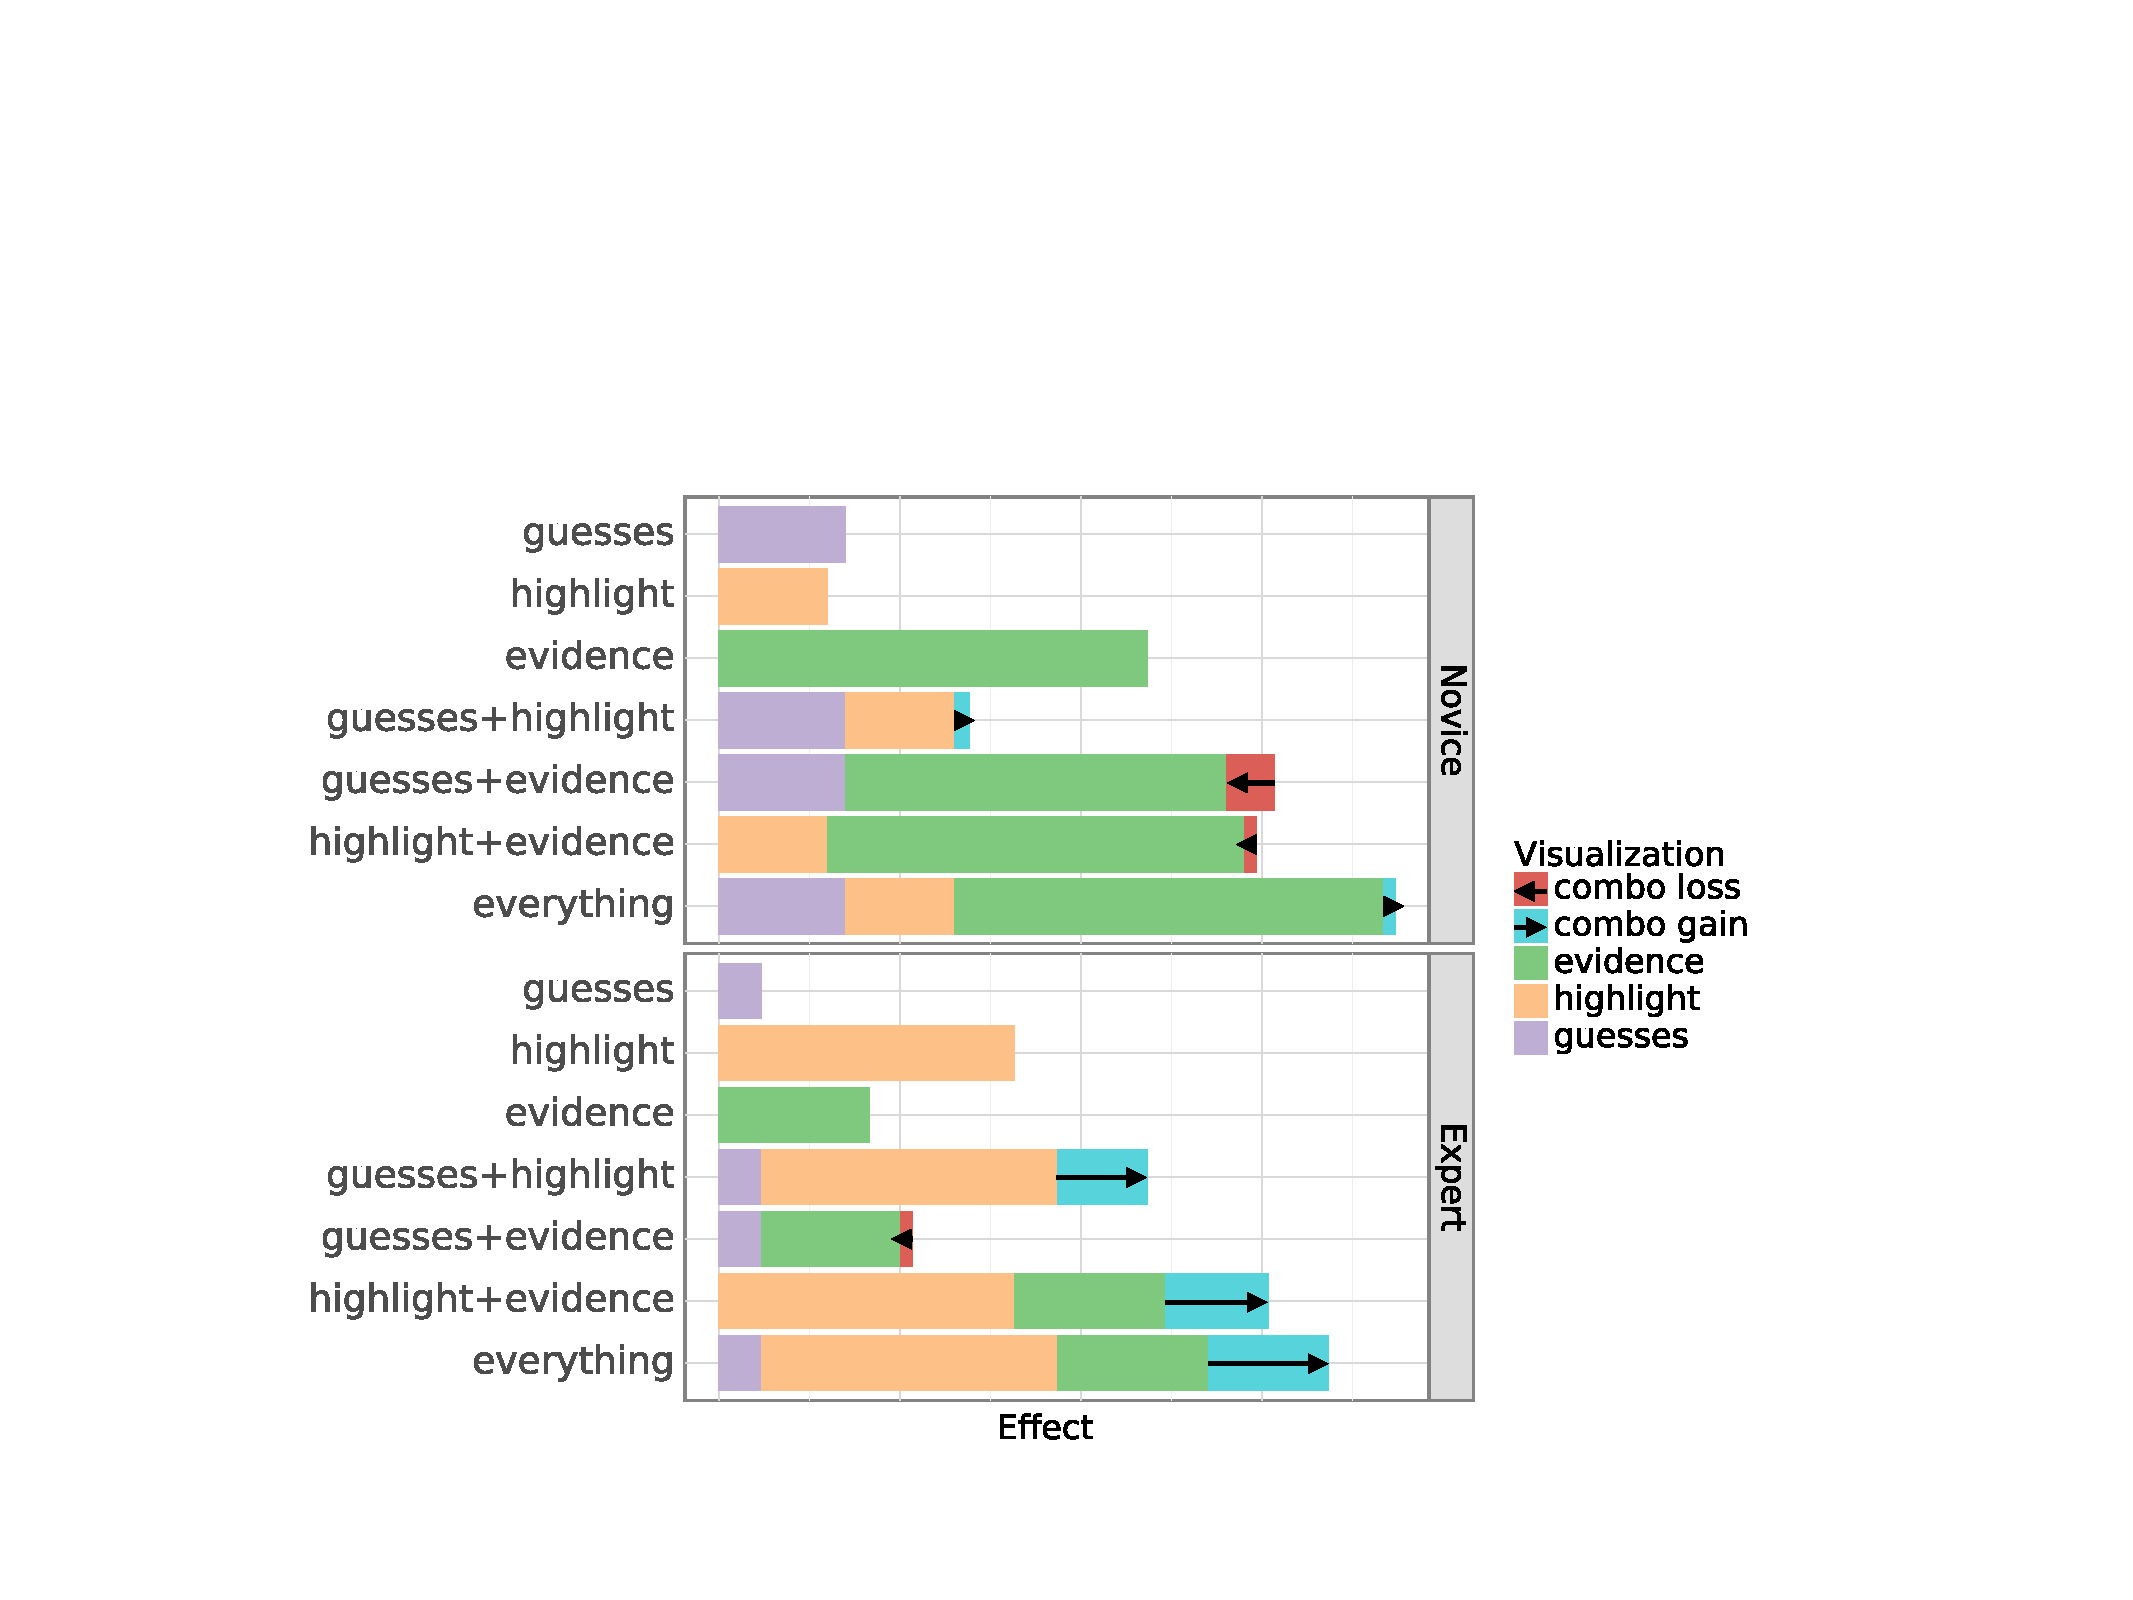
\includegraphics[width=1.0\columnwidth]{coefs_new}
    \caption{\label{fig:coefs} Coefficients of the linear regression
    showing the effects of interpretations, for novices (above) and
    experts (below).
    Higher value means an interpretation improves player accuracy.
    In addition to the individual interpretations, \emph{combo gain}
    and \emph{combo loss} capture the additional effect of combining
    multiple interpretations. \emph{Highlight} and \emph{Evidence}
    are effective for both novices and experts; combining leads to
    more positive effect for experts than novices, potentially because
    experts can process more information in limited time.}
\end{figure}

\begin{figure}[t]
    \centering
    \textbf{Effect of player ability}\par\medskip
    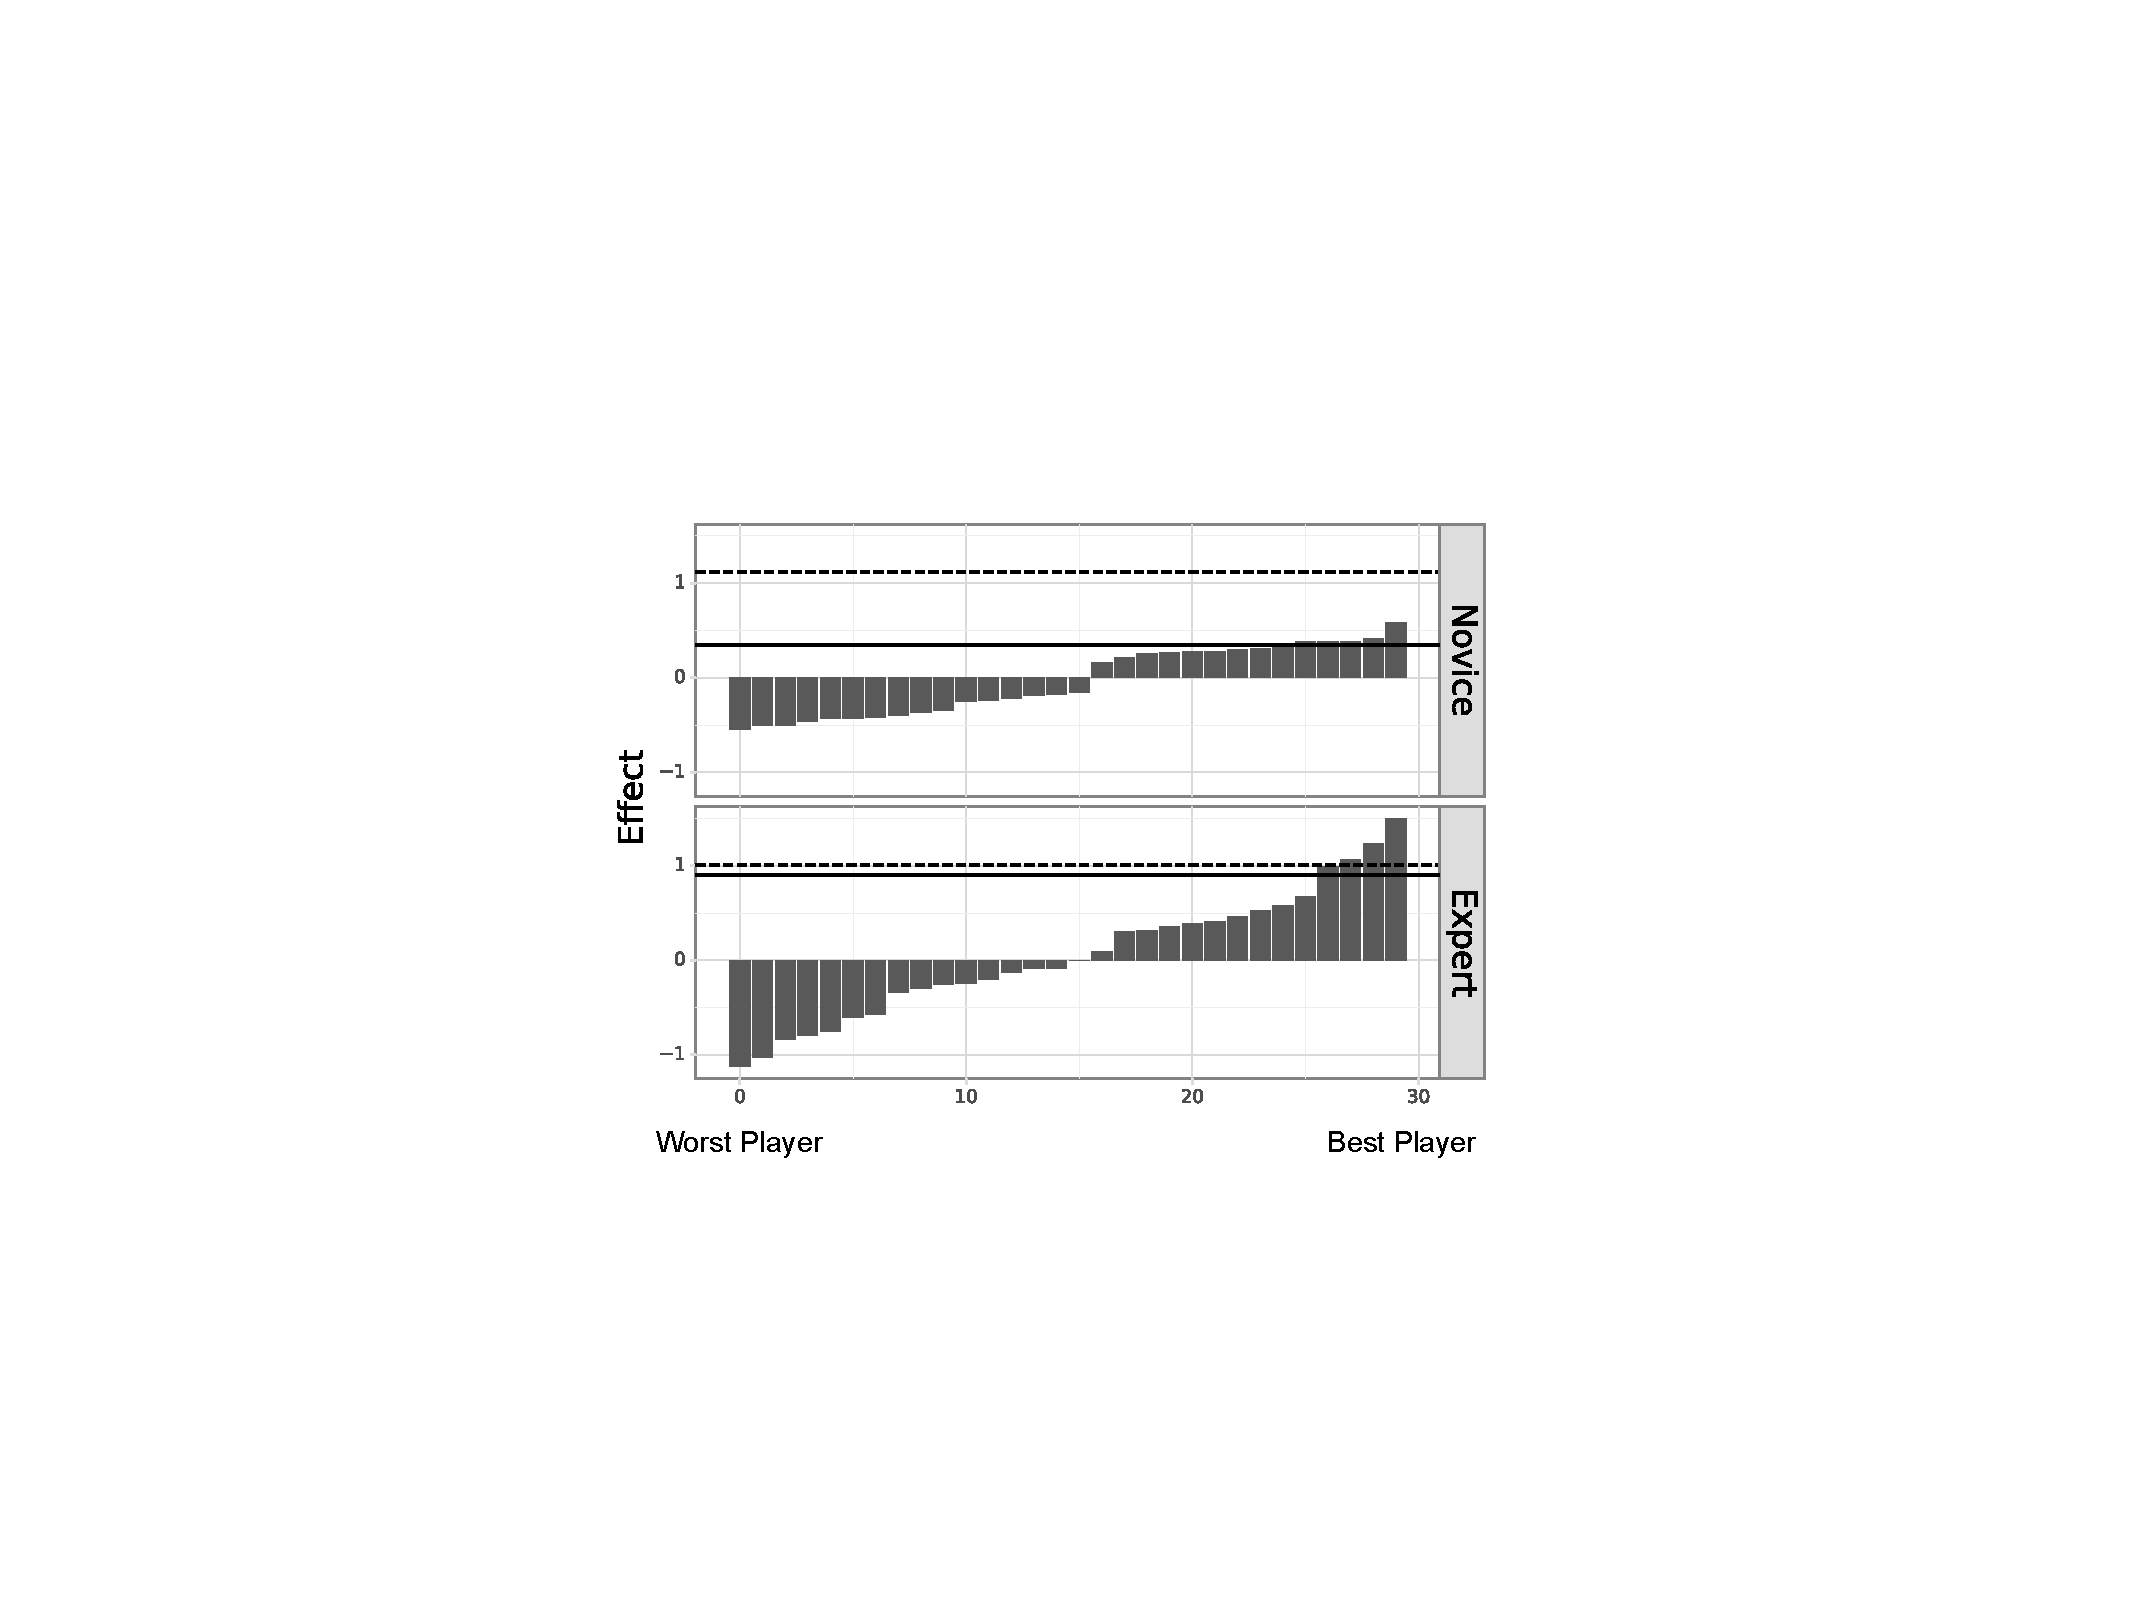
\includegraphics[width=.7\columnwidth]{u_coefs_new}
    \par\medskip
    \textbf{Effect of question difficulty}\par\medskip
    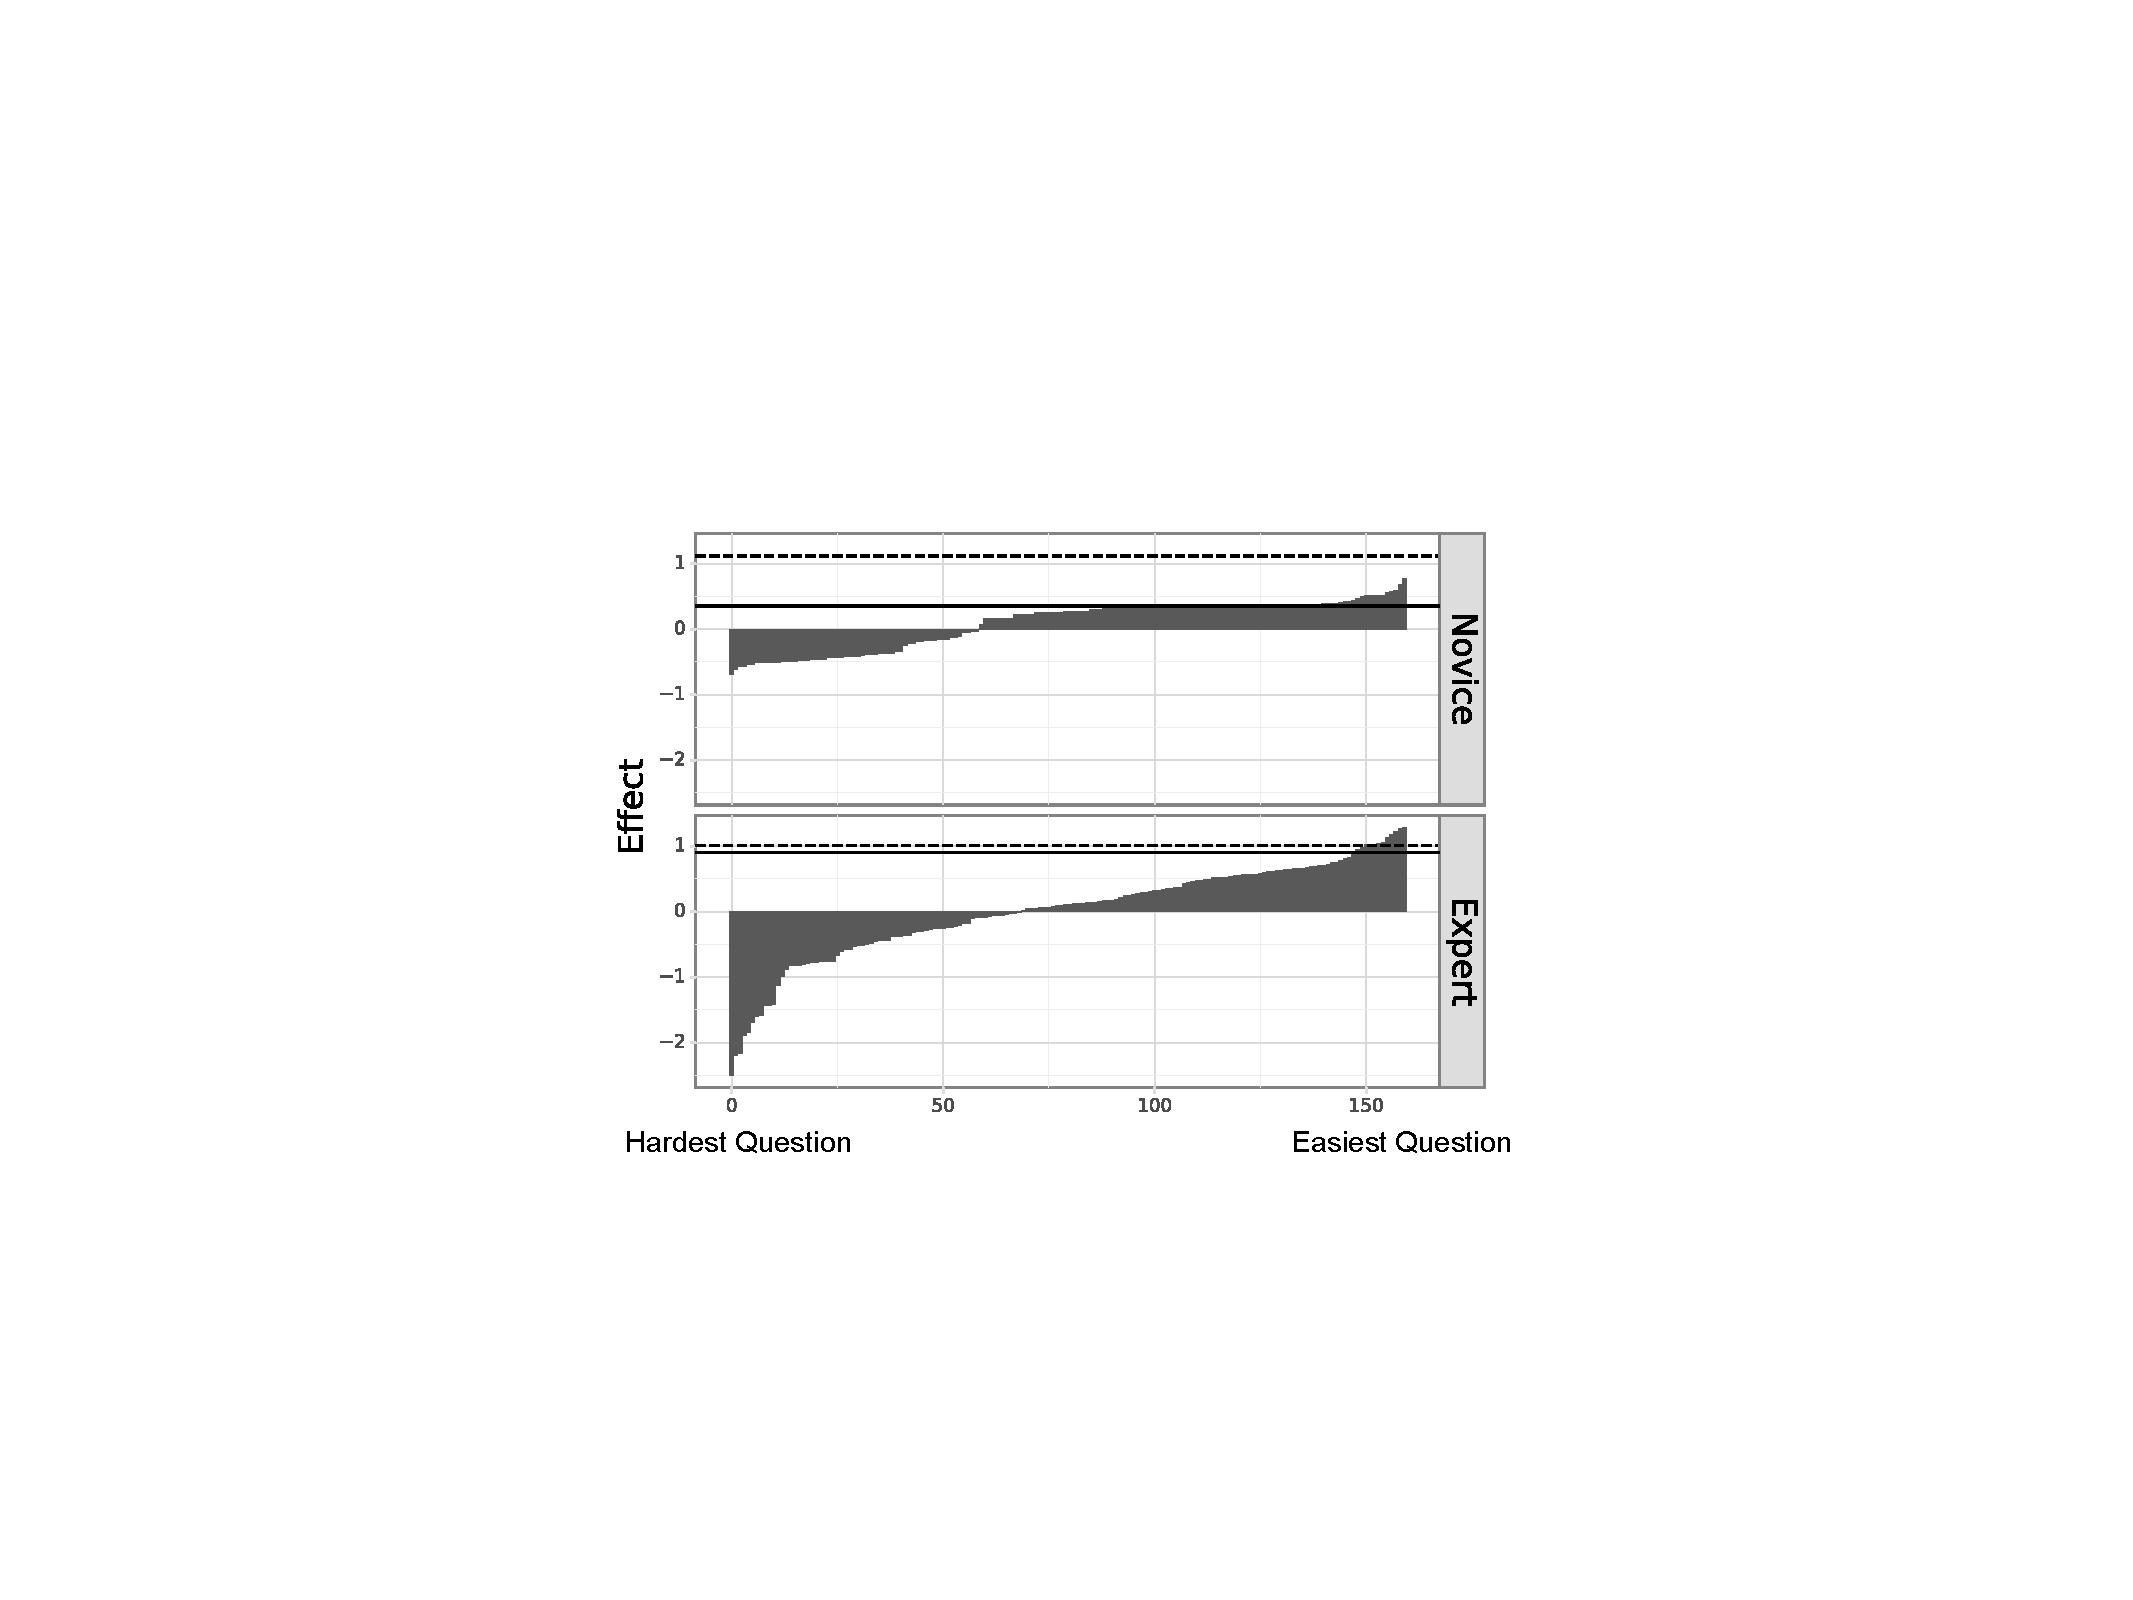
\includegraphics[width=.7\columnwidth]{q_coefs_new}
    \caption{\label{fig:uq_coefs} Effect of player ability (above) and
    question difficulty (below) from the regression analysis. Solid
    horizontal lines show the bias term that captures the baseline
    accuracy without any help from the computer;
    dashed lines show the effect of combining all
    interpretations.  Experts have a higher average accuracy; they are
    also less affected by interpretations.}
\end{figure}

% \begin{figure}[t]
%     \centering
%     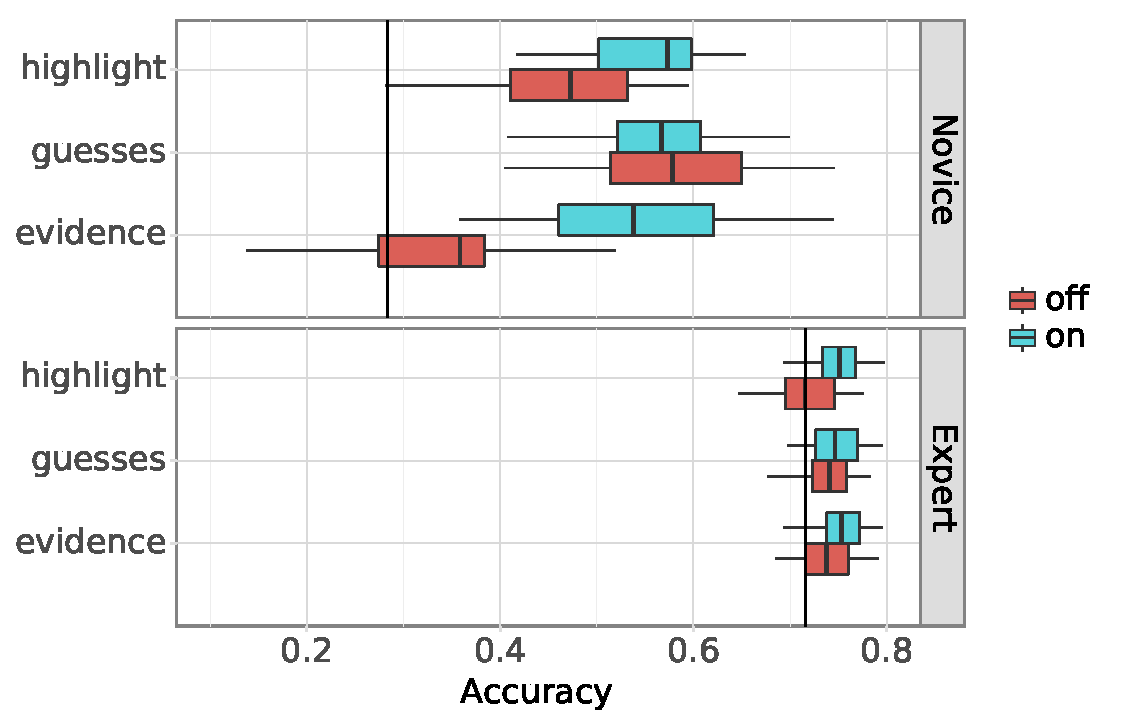
\includegraphics[width=\columnwidth]{tools_acc}
%     \caption{\label{fig:tools_acc} Accuracy of novices (above) and
%     experts (below), with and without each interpretation. One
%     interpretation being \emph{On} means that the interpretation is
%     shown to the players (possibly in combination with others); other
%     interpretations can still be used if one of them is \emph{Off}.
%     Vertical bars show the baseline accuracy without any
%     interpretation.
%     Unsurprisingly, experts show higher performance than novices and
%     are more consistent. Among the interpretations, evidence
%     significantly improves novice performance.}
% \end{figure}

\begin{figure}[t]
    \centering
    \textbf{Distribution of buzzes}\par\medskip
    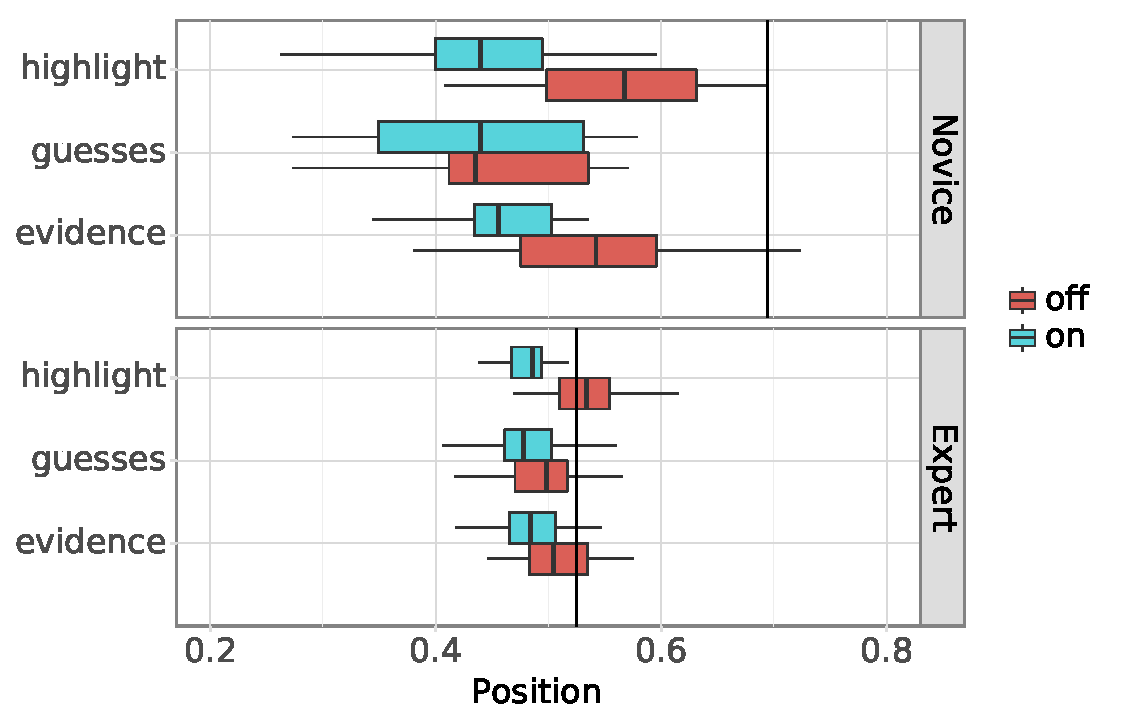
\includegraphics[width=\columnwidth]{tools_buzz}
    \caption{\label{fig:tools_buzz} Average buzzing position (relative
    to question length) of novices (above) and experts (below),
    with and without each interpretation. The goal is to buzz as early
    as possible.
    Vertical bars show the baseline buzzing position without any
    interpretation.
    % Like Figure~\ref{fig:tools_acc},
    Experts are better and more consistent.
    Among the interpretations, \emph{Highlight} is
    most effective in helping both novices and experts answer faster.}
\end{figure}

\begin{figure}[t]
\centering
\textbf{Aggressiveness of novice buzzes}\par\medskip
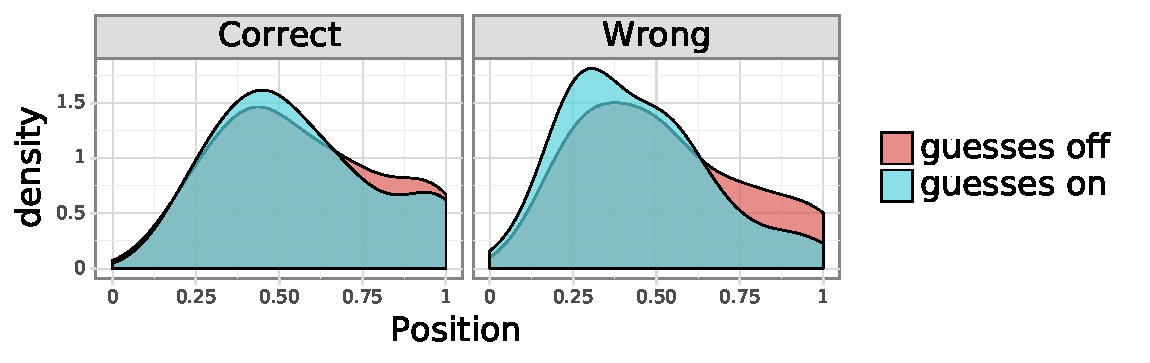
\includegraphics[width=.8\columnwidth]{novice_form_guesses}
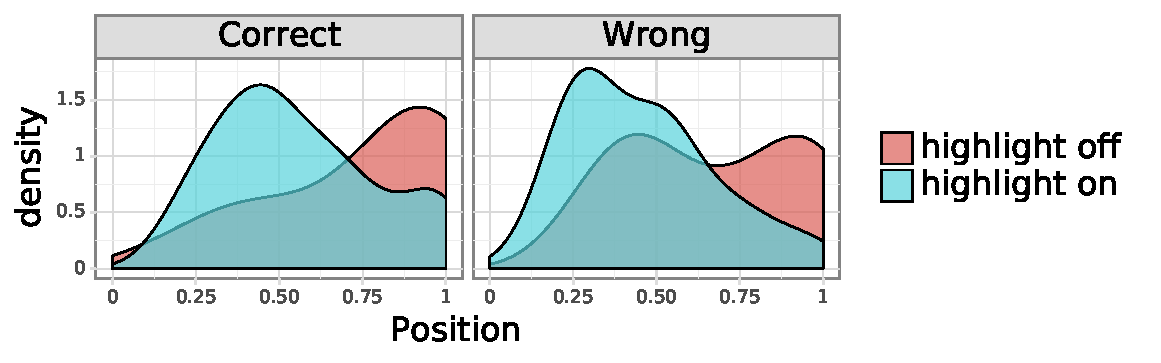
\includegraphics[width=.8\columnwidth]{novice_form_highlight}
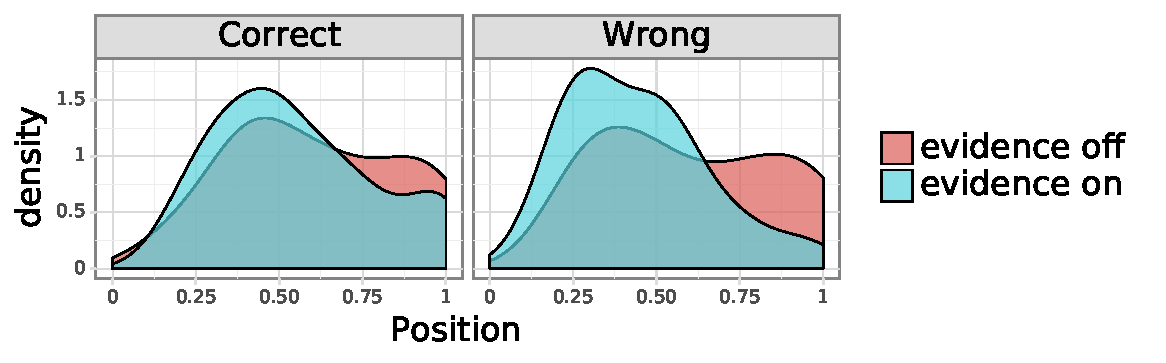
\includegraphics[width=.8\columnwidth]{novice_form_evidence}
\caption{\label{fig:aggressive_novice} The distribution of buzzes of
    novices on correct guesses (left) and wrong guesses (left); colors
    indicate if each interpretation is enabled; positions are
    normalized by question length.  With interpretations, novices are
    significantly more aggressive, but also get more questions correct
    earlier. \emph{Highlight} is the most effective.}
\end{figure}

\begin{figure}[t]
\centering
\textbf{Aggressiveness of expert buzzes}\par\medskip
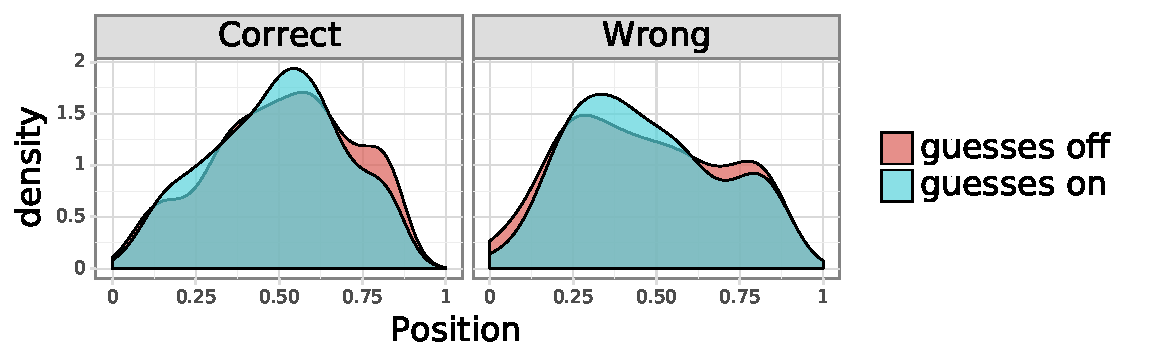
\includegraphics[width=.8\columnwidth]{expert_form_guesses}
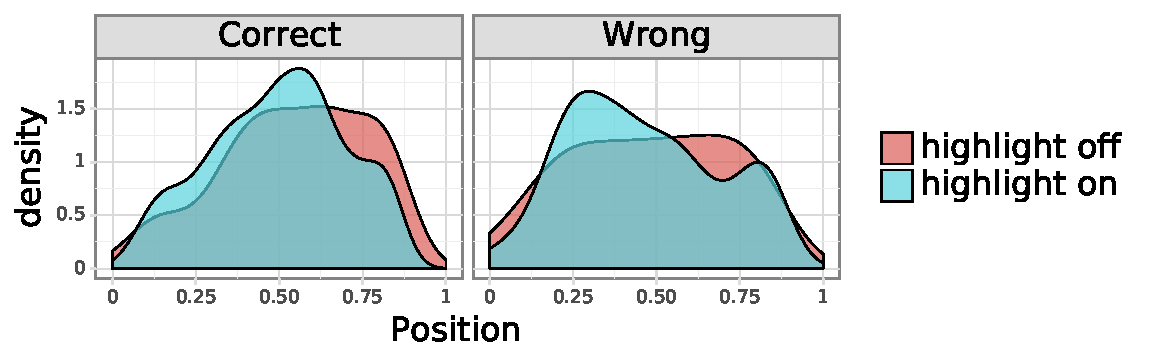
\includegraphics[width=.8\columnwidth]{expert_form_highlight}
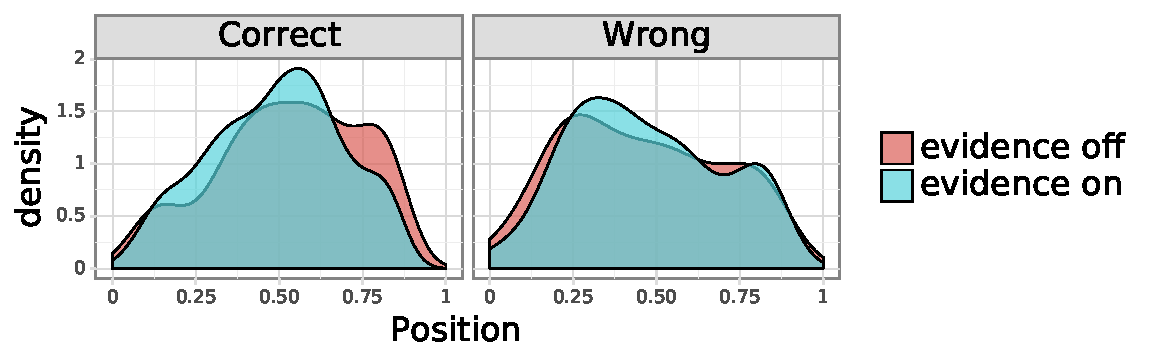
\includegraphics[width=.8\columnwidth]{expert_form_evidence}
    \caption{\label{fig:aggressive_expert} The distribution of buzzes
    of experts on correct guesses (left) and wrong guesses (left);
    colors indicate if each interpretation is enabled; positions are
    normalized by question length.  Experts are not significantly
    more aggressive with interpretations, but they did get more answers
    correct earlier.}
\end{figure}

% 1. overview of what we do in this section
With data collected from game plays, our primary goal is determine if
the interpretations are helpful or not, and how experts and novices
used them differently.
We first do a regression analysis to
quantitatively determine how much each condition affects the
accuracy of the players; then we break down the results to see
how the players behave differently under the conditions, specifically
how aggressive they are; we also look at specific cases where some
interpretation consistently succeeded or failed to convince multiple
players of the model prediction.

% 2. raw data description, using all numbers here for consistency
After filtering players who answer very few questions, we arrive at
30 experts that answer 1983 questions, and 30 novices that answer
600 questions. Turkers usually stopped after answering the required
twenty questions, but many experts kept on playing. Among all players,
seven experts answer all 160 questions.

\subsection{Regression Analysis}

% 3. motivate regression analysis
Whether a player can answer a question correctly is determined by
several factors: the player's innate skill, the difficulty of the
question, the aid of some interpretation, or the competitive level (in
expert setting).  To tease apart these factors we follow
Narayanan~\etal{}~\cite{narayanan2018humans} and apply a regression
analysis.

\begin{table}
\begin{tabular}{l|l}
\multirow{5}{*}{\begin{tabular}[c]{@{}l@{}}Interpretation\\ (8)\end{tabular}} & none, guesses, highlight, evidence,     \\
                                                                              & guesses + highlight,                    \\
                                                                              & guesses + evidence,                     \\
                                                                              & highlight + evidence,                   \\
                                                                              & guesses + highlight + evidence          \\ \hline
\multirow{2}{*}{Player (30)}                                                  & player IDs                              \\
                                                                              & (separate for experts and novices)      \\ \hline
Question (160)                                                                & question IDs                            \\ \hline
\multirow{5}{*}{Others (3)}                                                   & buzzing position                        \\
                                                                              & (relative to question length),          \\
                                                                              & number of active players (expert only), \\
                                                                              & current accuracy of the top             \\
                                                                              & active player (expert only)
\end{tabular}
\caption{\label{table:features} Our four sets of features used in
regression analysis. Numbers in the parentheses indicate the number of
features in that set.}
\end{table}

% 4. features
We describe these factors using the four sets of features listed in
Table~\ref{table:features}.
To capture the player's innate skill and the difficulty of the
question, we include the IDs of both in the feature set.  Each
combination of interpretations has its own features, for example,
\emph{guesses}, \emph{evidence}, and \emph{guesses+evidence} are three
independent features.  For game condition, the first feature is the
relative position in the question when the player buzzed (to
understand how interpretations affect buzzing position as an outcome
instead of feature, we use a separate analysis); for the expert
setting, we also include extra features to capture the
competitiveness: number of active players and the current accuracy of
the top active player.

% 5. the output
The we use a linear model to predict whether the player can answer the
question correctly.  Specifically, for each game record, we extract
the features and feed the vector as input to the linear model, which
then predicts the probability of a positive result; to train the
model, we compare the prediction against the ground truth, and update
the model with gradient descent.  We train this model on the game play
data, for experts and novices separately.

% 6. interpreting regression
The coefficients of the linear model then explains the
importance of the corresponding features: the probability of a
positive result increases with features with positive coefficients, which
means these features help the players. Similarly negative coefficient
means the features hurt the player accuracy.  To understand which
interpretations are most helpful to \qb{} players, we inspect the sign
and magnitude of their corresponding coefficients.

% 7. explain figure
Figure~\ref{fig:coefs} shows the effect of interpretations based on
regression coefficients: a high positive weight means the
interpretation is useful, zero means it is ineffective, and negative
means it is harmful.
It is not guaranteed that the strengths of multiple interpretations
are combined when they are displayed at the same time.
This is due to confounding factors such as information load---the
player might feel distracted when too much information is displayed on
the interface and thus perform worse.
The additional effects of combining
interpretations are ``combo gain'' and ``combo loss''
(Figure~\ref{fig:coefs}).
For example, combining guesses and evidence has a negative effect on
novices; the loss is computed by comparing the ``guesses+evidence''
coefficient with the arithmetic sum of the ``guesses'' and
``evidence'' coefficients.

% 8. findings about experts vs novices
The interpretation that helps novices is not the same as what helps
experts.  For experts, highlight is the most helpful individual
interpretation, while for novices, evidence is the most helpful. For
experts, the combination of highlight and evidence achieves extra
gain, which is reasonable because this combination adds
highlights to the evidence, making the contrast more intuitive.
However, the same combination does not show additional benefit for
novices, potentially due to information overload.

% 9. non-concrete finding
We hypothesize that the main difference between experts and novices is
that experts can use evidence more effectively. 
Question highlighting requires less
multitasking than evidence: players have to look away from the
question they need to answer to take in the evidence.  \qb{} players
likely know when they can glance down to related training data and can
also determine whether the training data are helpful.

% 10. non-interpretation factors
To understand how much variance players display in their skill and
questions in their difficulty, we show their corresponding
coefficients (Figure~\ref{fig:uq_coefs}). The solid horizontal line
shows the baseline accuracy of that player group without any
interpretation (the bias term---or the intercept---of the linear
model). Experts show a higher baseline accuracy, which is not
surprising since they are experts; they also show a larger variance
in accuracy within the group, potentially due to the competitive
environment; they are also more sensitive to the difference in
question difficulty.
To compare these factors against the interpretations, we
show with the dashed horizontal line the combination of all three
interpretations. Experts are less sensitive to the interpretations,
potentially due to a higher confidence in their own guesses.

\subsection{How Interpretations Change Player Behavior}

% 11. motivate the analysis of buzzing behavior
The regression analysis provides a quantitative comparison between all
interpretations in how they affect the player accuracy. However,
accuracy alone does not tell the full story of how they play the
game. This section describes how each
interpretation affects the behavior of the players and how the effect
differs for novices and experts.  Ideal players should be both
aggressive and accurate: seeing very few words and answering
correctly. Interpretations should help them reach this goal.

% 12. buzzing position with and without
Figure~\ref{fig:tools_buzz} show the
average buzzing position of each player group with and without each
interpretation.
% The effect of each
% interpretation on the accuracy of experts and novices concurs
% (Figure~\ref{fig:coefs}).
Novices buzz much later than experts when no interpretation is enabled
(comparing the solid vertical bars), but buzz at about the same point
as experts when interpretations are enabled, despite a lower accuracy
(Figure~\ref{fig:uq_coefs}). This suggests that the novices are too
trusting in the computer teammate, and end up playing too aggressively
for their skill level.

% 13. buzzing position density
We see a similar trend when we plot the density 
of buzzing positions (experts in Figure~\ref{fig:aggressive_expert}
and novices in Figure~\ref{fig:aggressive_novice}). In all settings,
the density shifts earlier: players are more aggressive with
interpretations, especially for novices, which is consistent with
Figure~\ref{fig:tools_buzz}. The interpretations allow players to
answer correctly earlier. Especially for novices with
highlights, the distribution of correct buzzing positions shifts
significantly earlier in the questions.

% 14. novices are too trusting
Although novices are helped by visualizations, these visualizations
are not enough to help them discern useful help from misleading help.
Novices are too aggressive at the start of the question with
visualizations: they trust the predictions of the system too much.
While experts mentally tune out bad suggestions, novices
are less discerning.  Visualizations thus 
must also convey whether they should be trusted, not just what answer
they are suggesting.

\subsection{Successes and Failures of Interpretations}

We now examine specific cases where interpretations help or hurt
players.

\begin{figure}[t]
\centering
\tikz\node[fill=white!70!colorsquad,inner sep=1pt,rounded corners=0.3cm]{
\begin{tabular}{p{0.46\textwidth}}
\emph{Question}:\\
(This essay) was composed after its author \textbf{refused} to
pay a \textbf{poll tax} to support the \textbf{Mexican-American}
\textbf{war}, and its ideology inspired Martin Luther King, Jr.\
and Mohandas Gandhi. \\

\emph{Evidence}:\\
him to pay six years of delinquent \textbf{poll tax}. Thoreau
\textbf{refused} because of his opposition to the
\textbf{Mexican-American War} and slavery, and he spent a night
in jail because of this refusal.
\end{tabular}
}; % end of tikz node
\caption{\label{fig:success} Interpretations that help players answer
a question on \underline{Civil Disobedience} correctly.  With the
shown part of the question, three experts answer correctly with the
evidence; no expert answer correctly without.}
\end{figure}

Figure~\ref{fig:success} shows an example where interpretations enable
players to answer correctly. A total of twelve expert players
answered the question, and eight answered correctly. The
earliest an expert can answer correctly without the evidence was at 72\%
of the question, while the three experts with the evidence all
answer correctly before 50\%. With the evidence and highlight,
players can infer from the keywords that the author is
Thoreau and that the guess is likely correct.  The computer shows
a salient training example and is effective in convincing the players
that the retrieved evidence is correct.

\begin{figure}[t]
\centering
\tikz\node[fill=white!70!colorsnli,inner sep=1pt,rounded corners=0.3cm]{
\begin{tabular}{p{0.46\textwidth}}
\emph{Question}:\\
A \textbf{book} by this man was first published with a
\textbf{preface} by Andreas Osiander titled \textbf{Ad Lectorem}.
\\
\emph{Evidence}:\\
the \textbf{Ad Lectorem} \textbf{preface} to Copernicus's
\textbf{book} was not actually by him.
\end{tabular}
}; % end of tikz node
\caption{\label{fig:fail_to_convince} Interpretations that fail to
    convince players.  Three expert players, when presented with the
    interpretation (some question text and evidence omitted), rejected the
    computer's correct guess (\underline{Copernicus}) and answered
    differently.}
\end{figure}

Figure~\ref{fig:fail_to_convince} shows a failure to convince,
where the combination of highlight and evidence fails to convince the
player of the computer's \emph{correct} guess: three expert players
rejected the computer's prediction and provided different answers,
relatively early in the question (before 50\%). The information
provided by the evidence is that Copernicus has a book with a
preface named Ad Lectorem, this piece of evidence strongly supports the
computer's guess \underline{Copernicus}.  However, it is expressed
differently than the question, with an unrelated but confusing ``not''
in the middle of the sentence.

% \jbgcomment{There needs to be more of an in-depth analysis.  Find:
%
% \begin{enumerate}
%   \item A player who is so good that no interface element helps
%   \item A super easy question
%   \item A very difficult question
%   \item Questions that suddenly become answerable with additional evidence, show the evidence that made it answerable
% (many of these can be found by looking at outliers)
% \end{enumerate}
%
% }

% \begin{table}[t]
% \centering
% \begin{tabular}{lll|ll}
%           & \multicolumn{2}{c|}{Accuracy}                           & \multicolumn{2}{c}{Position}                           \\
%           & \multicolumn{1}{c}{With} & \multicolumn{1}{c|}{Without} & \multicolumn{1}{c}{With} & \multicolumn{1}{c}{Without} \\ \cline{2-5}
% Guesses   & 0.7481                   & 0.7434                       & 0.5817                   & 0.5981                      \\
% Highlight & 0.7506                   & 0.7182                       & 0.5839                   & 0.6306                      \\
% Evidence  & 0.7487                   & 0.7380                       & 0.5813                   & 0.6134
% \end{tabular}
% \caption{Average accuracy and buzzing position (divided question length),
%     with and without each tool. Lower value in buzzing position indicates more
%     aggressive playing.}
% \label{table:form_acc_pos}
% \end{table}

\section{Discussion}
\label{sec:discussion}

% \fscomment{Need to explain in more detail, but the main takeaways are
%
% \begin{itemize}
%     \item our evaluation is a good extrinsic and application-grounded
%         evaluation
%     \item the effectiveness of interpretations varies with different
%         inputs and human users of different skill levels.  this
%         suggests the possibility of making the interpretations more
%         useful by automatically selecting ones to show based on the
%         input, and adapting to specific human user. RL or bandit
%     \item when computer performance is higher than human,
%         interpretation should pay more attention to showing
%         uncertainty
% \end{itemize}
% }

% \jbgcomment{I've been moving stuff here that delayed the point in
%   previous sections.  It's not well integrated or organized}
%
% \jbgcomment{Should have explicit design recommendations for people
%   building human in the loop interfaces}

% \subsection{Experts vs.\ Novices}
% In our cooperative setting, experts and novices use model
% interpretations differently.  Novices tend to be too trusting, playing
% much more aggressively when visualizations are enabled
% (Figure~\ref{fig:tools_buzz}).
% Interpretations that require less processing appear more useful to
% experts (Figure~\ref{fig:coefs}).
% For tasks where computer performs on the same level as human experts
% but shows different strengths,
% interpretations should be intuitive, easy to
% process.
% An unstructured saliency mapping
% over input features might not be effective enough
% (Figure~\ref{fig:fail_to_convince}).

The evaluation we present is grounded in a realistic setting, but also
task-specific. This section discusses how our method can be directly
applied to other settings, its limitations, and how we can incorporate
other components such as an eye tracker to our framework for a more
fine-grained assessment of interpretability.

\subsection{Forms and Methods of Interpretation}

Interpretations take on many forms, and within each form we have multiple
methods to generate the interpretation. For example, to highlight
salient input features for image classification, we can use variants
of input gradient~\cite{baehrens2010explain, simonyan2013deep}.
To optimize the generalizability of our results (despite being
task-specific) and demonstrate the flexibility of our method, we
focus on a comparison between forms of interpretation. To
select one method of each form, we choose a
high-performance linear model for its canonical interpretations.  Our
evaluation framework, including the interface and the regression
analysis, can be directly applied to a different comparison---one
between multiple methods of the same form.  This comparison is
particularly useful in the case of neural models, where all existing
interpretations are some approximation, and the evaluation of
how faithful they are to the model is crucial.


\subsection{Intrinsic and Extrinsic Evaluation}

Our approach is an extrinsic evaluation~\cite{narayanan2018humans}. The
task is played by thousands who compete in regularly.  Using
\qb{} allows a contextual, motivated evaluation of whether an
interpretation is useful. In contrast, intrinsic evaluation relies on
the interpretation alone. It is more direct but limited. In tasks
where no ground-truth explanation is available, the most tractable and
commonly used method is to construct ground-truth using a simpler
model as a benchmark for interpretability. For example, weights of linear models are
used for evaluating input highlight
explanations~\cite{li2016understanding,murdoch2018cd}.
This is restricted to tasks where the benchmark model performs
similarly to the complex model that requires interpretation, and it
does not work in application-grounded setting
(Section~\ref{sec:eval_qb}).

Extrinsic evaluations are hard to design, as they are affected by more
factors, especially humans' trust. When a user does not trust the
model and ignores it, the difference in the performance is not
affected by the explanations at all. Narayanan~\etal{}~\cite{narayanan2018humans} uses
``alien'' tasks to enforce trust, tasks that humans do not have
knowledge of. Our approach, in contrast, considers trust as an
inherent part of the cooperation: good interpretations should be
consistent and intuitive to convince humans to use it.

% generalizability
% 1. comparison between underlying algorithms
% 2. other tasks
% This paper focuses on comparing forms of
% interpretations, so we limited the experiment to one method in each
% form. However, our evaluation framework, the interface, and the
% experimental setup can be naturally adapted to other comparisons, for
% example, between different underlying algorithms within each
% form, or between different models with interpretation methods fixed.

\subsection{Generalizing to Other Tasks}
Our method can be applied to natural language tasks other than
\qb{}, although \qb{}'s characters make it uniquely suitable.  To use
our interface for some other text classification task, for example
sentiment analysis or spam detection, one can convert the task into an
incremental version where the input is shown
word-by-word. Time limitation or competition can be added to
encourage the users to pay attention to
visualizations~\cite{narayanan2018humans}. One task
related to \qb{} has wide real world application: simultaneous
interpretation (or simultaneous translation, not to be
confused with model interpretation). Interpreters need to trade off
between accuracy and delay, much like \qb{}ers need to balance
accuracy and aggressiveness. The underlying mechanism of the
\abr{qanta} buzzer~\cite{he2016opponent} also resembles how
simultaneous translation systems handle this
trade-off~\cite{grissom:he:boyd-graber:morgan-2014}.

% limitations
% 1. UI design, equal exposure (placement)
% 2. ordering of questions, learning curve
\subsection{Limitations}
First, because we
compare visualizations individually and in combinations, their
placement is fixed to avoid confusing the players. The fixed
placement leads to uneven exposure to the users, so they might pay
less attention to some visualizations than others. If we focus on
individual visualizations, one way to resolve this issue is to display
the interpretation in a single fixed location, for example below the
question area. This would lead to a fair display of different
visualizations without confusing the users. However, one single
location might not suit all visualizations: for example, input
highlight should collocate with the input, while evidence is best
displayed next to the input for comparison.

Visualizations displayed on our interface change from question to
question, and the randomization (Setup)
might confuse the users. Before answering questions, each user sees
a tutorial that walks through the components of the interface,
but this can be improved by a set of warm-up questions to familiarize
the users of the interaction, which we will implement in future
studies. In addition, we can randomly sort the questions instead of
the visualizations, so the users see the same layout for multiple
questions, reducing context switches and consequently the cognitive
load.

Another limitation of our study is that, when a player's performance
improves with some interpretation, we cannot tell how much of that
improvement comes from the player using that interpretation.
We cannot derive causality from correlation. The key
missing factor is how much attention the player gave the interpretation,
and how much the decision is based on that. The attention the player
gave each interpretation could be measured using an eye tracker, and we
leave this to future work.


% \subsection{A Question of Trust}
%
% However, we believe that trust should not be separated from the
% evaluation, as it is an inherent part of a human-in-the-loop
% system. There will always be a varying degree of trust in the system
% when it is used in the real world. And to keep the end-to-end
% assessment consistent with the real world, we should not force trust
% in our extrinsic evaluations. Moreover, it would be ideal if we can
% simlutate different degrees of human trust to make the evaluations
% more realistic and accurate.
%
% Trust can be affected by many factors: accuracy of the system,
% consistency of the explanation, and also external rewards. Reward
% structures of competitive environments can incentivize humans to use
% the model outputs in a certain way.  For example, when a large
% negative reward is given on incorrect prediction, the users would be
% encouraged to be more careful and less reliant on the model. By tuning
% the external rewards, we can achieve more fine-grained control,
% without resorting to ``alien" tasks.
%
% One benefit of our framework as a competition is that we can adjust
% players' loss function through the \qb{} scoring mechanism.  For
% example, we can offer ``power'' points for early answers (typically in
% competition) or increase the penalty for getting questions wrong
% (sometimes seen with larger player pools).  This can encourage players
% to depend on the visualization more (increasing rewards) or to be more
% skeptical (increasing penalties).

%% \subsection{Trust Factor and Threat to Validity}
%% As mentioned in Section~\ref{sec:eval_qb}, degree of trust can be adjusted by
%% tuning the reward structure, but we cannot guarantee consistent trust across
%% player. The main threat to the validity of our results is the variance in player
%% baseline performance, difficulty of questions, and degree of trust. We plan to
%% collect more data, which would allow the regression analysis to factor out these
%% variance more accurately.

% \subsection{Persuasive vs. Informative}

\subsection{Future Work}

While we focus on broad categories of interpretations to reveal that
some visualizations are more effective than others (e.g., highlighting
is more useful than guess lists), we can also use this approach to
evaluate specific highlighting methods in a task-based setting.  This
can help reveal how best to choose spans for highlighting, which words are best
suited for highlighting, and how to convey uncertainty in
highlighting.

While our evaluation focuses on the downstream task, we can expand
our analysis to measure how much users look at visualizations and in
what contexts (e.g., with an eye tracker).  This would reveal situational usefulness of
visualization components; if, for example, highlighting were only
useful to distinguish when two guesses had similar scores, we could
decrease cognitive load by only showing highlights when needed.

A tantalizing extension is to make these modifications automatically,
using the reward of task performance to encourage a reinforcement
learning algorithm to adjust interface elements to optimize
performance: such as changing font sizes, setting buttons for users to
explicitly agree or disagree with model predictions, or modifying the
highlighting strategy.

% \subsection{Other Tasks}
%
% Another possible extension is to convert any language task into a
% competitive version for interpretation evaluation. Natural language is
% inherently sequential, so converting the tasks into incremental
% versions is trivial. Then we can turn them into competitive games. For
% example, predicting the verb in simultaneous translation is very
% similar to the \qb{} answering task~\cite{Grissom-14}.  By comparing
% the evaluation in both incremental and non-incremental settings, we
% might be able to quantitatively determine whether the competitiveness
% achieved by this conversion indeed lead to more realistic and accurate
% evaluation.
%
% Previous work have studied the evaluation of interpretation in
% cooperative~\ref{Antunes2008StructuringDF}, and
% application-grounded~\ref{williams2016axis} settings. However, our
% work is the first to conduct application-grounded evaluation in
% natural language processing domain.

\section{Conclusion}
\label{sec:conclusion}

We propose and demonstrate an evaluation of interpretation methods in a
human-\abr{ai} cooperative setting. We focus on the natural language
domain and use a question answering task derived from a popular trivia
game, \qb{}.
Our experiments with both experts and novices reveal how they trust and
use interpretations differently, producing a more accurate and
realistic evaluation of machine learning interpretability. Our results
highlight the importance of taking the skill level of the target user
into consideration, and suggests that, combining
interpretations more intelligently and adapting to the user, we can
further improve the human-\abr{ai} cooperation.


\begin{acks}
We thank the anonymous reviewers for their insightful and constructive
comments.  Additionally, we would like to thank Alison Smith, Leah
Findlater, Hernisa Kacorri, Alina Striner, and Andreas Mathisen for
their valueble input.
This work was supported NSF Grant \abr{IIS}-1822494 and subcontract to
Raytheon BBN Technologies by DARPA award HR0011-15-C-0113.
Any opinions, findings,
conclusions, or recommendations expressed here are those of the
authors and do not necessarily reflect the view of the sponsor.

\end{acks}

\bibliographystyle{style/ACM-Reference-Format}
\bibliography{bib/journal-full,bib/jbg,bib/fs}

\end{document}
